\documentclass{report}

% Language setting
% Replace `english' with e.g. `spanish' to change the document language
\usepackage[UKenglish]{babel}
\usepackage{url}

% Set page size and margins
% Replace `letterpaper' with `a4paper' for UK/EU standard size
\usepackage[letterpaper,top=2cm,bottom=2cm,left=3cm,right=3cm,marginparwidth=1.75cm]{geometry}

% Useful packages
\usepackage{amsmath}
\usepackage{graphicx}
\usepackage[colorlinks=true, allcolors=blue]{hyperref}
\usepackage{float}
\usepackage{indentfirst}
\usepackage{caption}
\captionsetup{justification=centering}
\usepackage[autostyle]{csquotes}
\usepackage{wrapfig}
\usepackage{booktabs}
\usepackage{tabularx}
\usepackage{array}

\bibliographystyle{IEEEtran}
\setlength{\parindent}{15pt}

\title{Thinking Inside the Box: Efficient Privacy-First Architecture for Distributed Reasoning using Federated Large Language Models}
\author{Viacheslav Horbanov, CSC3094 Major Project and Dissertation in Computer Science}
\date{April 22, 2026, Newcastle University}

\begin{document}

% \maketitle

% \vspace{-2.5em}
% \begin{center}
% Word Count: 2303
% \end{center}


\maketitle

\section*{Executive Summary}
\addcontentsline{toc}{section}{Executive Summary}

\textbf{Problem.} Cross-silo institutions in regulated domains (banking, healthcare, legal) need to learn jointly from data that they cannot legally pool. Classical federated learning at LLM scale fails on bandwidth (approximately $16$~GB per client per round at fp16 for an 8-billion-parameter backbone) and silently degrades on utility when the silo-specific knowledge that drives the supervised task lives only in one institution.

\textbf{Architectural premise.} The Privacy-Utility-Efficiency Trilemma is not intrinsic to federated LLMs; it is a property of co-locating reasoning capacity and sensitive knowledge inside the same learnable parameters. Once the two are separated, reasoning lives in a shared low-rank adapter (FLoRA) and crosses the network; knowledge lives in a per-node graph store and never does.

\textbf{Three headline numbers, all reproducible from \texttt{benchmark-2026-04-02}.}
\begin{itemize}
    \setlength\itemsep{0em}
    \item \textbf{Utility.} FLoRA-with-RAG peaks at F1 score~$=0.805$, within $0.05$ of the centralised-flat upper bound of $0.852$, and is the closest federated approximation of the centralised utility ceiling in the six-condition benchmark.
    \item \textbf{Efficiency.} FLoRA's per-client per-round payload of $18.2$~MB is $882\times$ smaller than the McMahan-style fp16 reference. At a $100$~Mbps WAN link the per-round upload is $1.46$~seconds, while the per-round fit stage is $770$~seconds; bandwidth ceases to be a deployment constraint.
    \item \textbf{Privacy.} Membership-inference AUC stays in the $0.44$-$0.45$ band against a chance baseline of $0.50$ across every federated condition.
\end{itemize}

\textbf{Three contributions.} (1) The composition of FLoRA adapter federation with a bank-scoped local RAG retriever, evaluated end-to-end on the IBM AML task; (2) a Strategy-pattern graph layer (\texttt{KuzuGraphStore}, \texttt{NetworkXGraphStore}, \texttt{Neo4jGraphStore}) that lets the federation and RAG layers swap backends without code change; (3) a reproducible per-round per-client benchmark archive under git tag \texttt{benchmark-2026-04-02} that operationalises the audit trail expected by the UK and Canadian model-risk regimes (PRA SS1/23 and OSFI Guideline E-23).

\textbf{Three limitations stated up front.} The benchmark is single-seed; the privacy probe is a threshold-based proxy not a shadow-model attack; the IBM AML dataset is synthetic and cost projections inherit its class distribution. Each is treated explicitly in Section~\ref{sec:results:limits}.

\textbf{Cost of running it.} A full ten-round three-client federated training session consumes $6.42$~A100-hours; at on-demand A100 cloud pricing this is between USD~$6.87$ and USD~$26.25$ per session, or approximately USD~$357$-$1{,}365$ per consortium per year at a weekly retraining cadence. Compute is not the constraint on adoption.

\textbf{Reusability.} The architecture makes no assumptions about the underlying domain; the AML case is a study, not a specialisation. The same federation-plus-local-RAG pipeline retargets to healthcare, legal discovery, inter-hospital research, and cross-jurisdiction compliance by replacing only the ingestion layer and the retrieval-time prompt. The regulatory framing in Section~\ref{sec:meth:regulatory} is presented in the AML setting but applies, with the appropriate sector-specific instruments substituted in, to any of the above domains.

\begin{abstract}
\textbf{Problem and context.} Federated Learning (FL) was introduced to let institutions train shared machine learning models on data that they cannot legally pool: hospitals on patient records, banks on customer transactions, courts on case archives. Recent reasoning-capable Large Language Models (LLMs) have parameter counts of order $10^{10}$, which classical Federated Averaging (FedAvg) cannot transmit at acceptable cost; the literature formalises this as a Privacy-Utility-Efficiency Trilemma in which strengthening any one axis is paid for on the other two. The Anti-Money Laundering (AML) task is a natural test bed because the analytic signal sits in graph-structured transactions that span institutions, while privacy regulation forbids those institutions from pooling the data.

\textbf{Methodology.} ``Thinking Inside the Box'' resolves the trilemma by decoupling \textit{reasoning} from \textit{knowledge}: reasoning lives in a shared adapter trained federatively (FLoRA, Federated Low-Rank Adaptation), and knowledge lives in a per-node Retrieval-Augmented Generation (RAG) pipeline over a local graph store. The simulation runs three bank clients on the IBM AML dataset across ten federation rounds and six experimental conditions (three aggregators - centralised, FedAvg, FLoRA - crossed with two retrieval modes - flat, RAG), with utility, efficiency, and privacy reported on each round. The backbone is DeepSeek-R1-Distill-Llama-8B at 4-bit NF4 quantisation; only encrypted low-rank adapter deltas cross the privacy boundary.

\textbf{Results.} FLoRA-with-RAG reaches a peak F1 score score of $0.805$, within $0.05$ of the centralised-flat upper bound of $0.852$. Per-client per-round bandwidth is $18.2$~MB, an $882\times$ reduction over an fp16 FedAvg reference at 8-billion-parameter scale; a full ten-round three-client session consumes $6.42$~A100-hours at on-demand cloud pricing of USD~$6.87$ to USD~$26.25$ per session. Membership-inference AUC stays in the $0.44$-$0.45$ band across every federated condition against a chance baseline of $0.50$. The architecture is mapped explicitly onto five regulatory regimes (GDPR Articles 5(1)(c) and 25; FATF Recommendations 10, 11 and 20 with the UK Money Laundering Regulations 2017; USA PATRIOT Act \S~314(b); PRA Supervisory Statement SS1/23 and OSFI Guideline E-23; Sixth Anti-Money Laundering Directive 2018/1673), with each regulation tied to a specific design decision in the Methodology chapter.

\textbf{Limitations.} The benchmark is single-seed, so reported peaks and finals are point estimates rather than confidence intervals. The privacy probe is a threshold-based membership-inference attacker, weaker than a shadow-model construction. The IBM AML dataset is synthetic; the cost projections inherit its class distribution and may not transfer to a real bank's monitoring stream without recalibration. The architecture itself is domain-agnostic and is presented under the AML case study only.
\end{abstract}

\tableofcontents
\addcontentsline{toc}{section}{Table of Contents}

\section*{List of Acronyms}
\label{sec:acronyms}
\addcontentsline{toc}{section}{List of Acronyms}

The dissertation introduces each acronym in full on first use; subsequent occurrences use the bare acronym. The same expansions are listed here for the convenience of a reader who does not read in linear order.

\begin{tabularx}{\textwidth}{l X}
\toprule
\textbf{Acronym} & \textbf{Expansion} \\
\midrule
6AMLD & Sixth Anti-Money Laundering Directive (Directive (EU) 2018/1673) \\
AML & Anti-Money Laundering \\
AUC & Area Under the (ROC) Curve \\
CDD & Customer Due Diligence \\
F1 score & Harmonic mean of precision and recall (the binary classification metric named ``F1''; not Formula 1 motorsport) \\
FATF & Financial Action Task Force \\
FCA & Financial Conduct Authority (United Kingdom) \\
FedAvg & Federated Averaging \\
FFI & Federally Regulated Financial Institution (Canada) \\
FinCEN & Financial Crimes Enforcement Network (US Department of the Treasury) \\
FIU & Financial Intelligence Unit \\
FL & Federated Learning \\
FLoRA & Federated Low-Rank Adaptation \\
fp16, fp32 & 16-bit and 32-bit IEEE-754 floating-point precision \\
GB, MB, Mbps & gigabytes, megabytes, megabits per second \\
GDPR & General Data Protection Regulation (Regulation (EU) 2016/679) \\
HSM & Hardware Security Module \\
IBM AML & The Weber et al.~synthetic Anti-Money Laundering transaction dataset \\
IID & Independent and Identically Distributed \\
KV cache & Key-Value attention cache (LLM inference memory) \\
LLM & Large Language Model \\
LoRA & Low-Rank Adaptation \\
MIA & Membership Inference Attack \\
MLR 2017 & UK Money Laundering, Terrorist Financing and Transfer of Funds (Information on the Payer) Regulations 2017 (SI 2017/692) \\
MoE & Mixture of Experts \\
MRM & Model Risk Management \\
NF4 & 4-bit NormalFloat (QLoRA quantisation data type) \\
non-IID & Non-Independent and non-Identically Distributed \\
OOM & Out-Of-Memory \\
OSFI & Office of the Superintendent of Financial Institutions (Canada) \\
PEFT & Parameter-Efficient Fine-Tuning \\
PRA & Prudential Regulation Authority (Bank of England) \\
QLoRA & Quantised Low-Rank Adaptation \\
RAG & Retrieval-Augmented Generation \\
ROC & Receiver Operating Characteristic \\
SAR & Suspicious Activity Report \\
SS1/23 & PRA Supervisory Statement 1/23 (Model Risk Management Principles for Banks) \\
STR & Suspicious Transaction Report \\
SVD & Singular Value Decomposition \\
USD & United States Dollar (currency) \\
VRAM & Video Random Access Memory (GPU memory) \\
WAN & Wide Area Network \\
\bottomrule
\end{tabularx}

\chapter{Introduction}
\label{ch:introduction}

\section{Motivation and Context}

Large Language Models (LLMs) are increasingly deployed in domains where information sensitivity, regulatory constraints, and data sovereignty are paramount. Industries such as finance, healthcare, and education hold rich, analytically valuable records that could enable breakthrough artificial intelligence applications, yet centralising such records would violate privacy legislation and commercial confidentiality commitments. Within financial services this tension is acute. Anti-Money Laundering (AML) investigations depend on recognising transaction patterns that span multiple institutions, but regulations including the General Data Protection Regulation (GDPR) and national banking secrecy laws prohibit the bulk transfer of customer records between institutions. A bank observing suspicious behaviour in isolation may see only one segment of a structuring or layering chain that was deliberately fragmented across the interbank payment system. The analytical asymmetry between malicious actors, who coordinate freely across jurisdictions, and investigators, who cannot, is a long-standing weakness of centralised forensic pipelines.

Federated Learning (FL) was introduced specifically to address this asymmetry \cite{mcmahan2017communication}. In place of sharing raw data, participating institutions each train a local model on their private records and exchange only aggregated parameter updates. Since its formalisation in 2017, FL has enabled collaborative training across hospitals, smartphones, and banks without violating data residency constraints. However, the recent generation of reasoning-capable LLMs \cite{deepseek2025r1}, with parameter counts in the billions, exposes fundamental limitations in how classical federated optimisation scales to modern architectures.

\section{The Privacy-Utility-Efficiency Trilemma}

Deploying large reasoning models in a federated environment surfaces a three-way tension that the literature has formalised as the Privacy-Utility-Efficiency Trilemma \cite{plosone2023e0338822, allouah2023trilemma}. The three axes conflict as follows.

\begin{enumerate}
    \setlength\itemsep{0em}
    \item \textbf{Privacy.} Retaining raw records on-node precludes globally contextual reasoning; each model only sees its local slice of the world.
    \item \textbf{Utility.} Recovering global context by sharing data, shared representations, or dense feature aggregates erodes the privacy guarantee that motivated federation in the first place.
    \item \textbf{Efficiency.} Transmitting full LLM weight updates every round, as in naive Federated Averaging (FedAvg), consumes tens of gigabytes of network bandwidth per round per client. At production scale this is not merely inconvenient; it is infeasible.
\end{enumerate}

Existing approaches typically resolve the trilemma by trading one axis against another, as Figure~\ref{fig:concept-trilemma} illustrates. Differential privacy mechanisms strengthen the privacy axis at a direct cost to utility. Model compression and gradient quantisation reduce communication volume but introduce accuracy penalties that compound across rounds. Shared proxy datasets leak indirect information about the sources. The premise of this project is that the three axes need not be traded at all: they can be \textit{decoupled} by separating the component of the system that requires learning from the component that holds the sensitive information.

\begin{figure}[t]
    \centering
    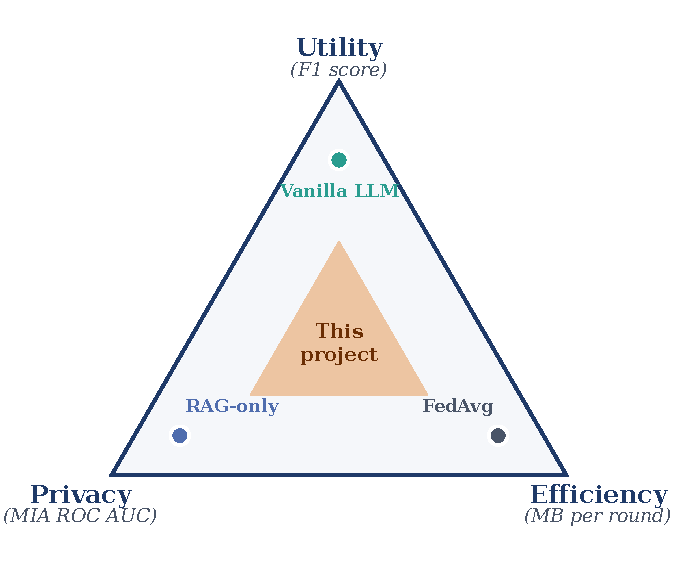
\includegraphics[width=0.72\linewidth]{res/fig-concept-trilemma.pdf}
    \caption[The Privacy-Utility-Efficiency Trilemma]{The Privacy-Utility-Efficiency Trilemma motivating the architectural design (Section~\ref{sec:meth:arch}). Existing federated designs sit on one edge of the triangle, trading one axis against another. This project targets the shaded interior by decoupling shared reasoning (FLoRA adapters) from local knowledge (per-node RAG), removing the direct competition between axes.}
    \label{fig:concept-trilemma}
\end{figure}

\section{Gap in Existing Approaches}

Three lines of research contribute independent pieces of a solution, but to date they have not been combined in a single architecture for federated reasoning over sensitive domains.

First, parameter-efficient fine-tuning techniques such as Low-Rank Adaptation (LoRA) \cite{hu2021lora}, its quantised variant QLoRA \cite{dettmers2024qlora}, and the federated extension FLoRA \cite{flora2024federated} reduce the trainable footprint of an LLM from billions of parameters to a rank-constrained adapter that is several orders of magnitude smaller. This addresses the efficiency axis directly. However, a LoRA adapter trained only on one bank's transactions carries only that bank's view.

Second, Retrieval-Augmented Generation (RAG) \cite{lewis2021retrievalaugmentedgenerationknowledgeintensivenlp} lets a language model condition its output on external context retrieved at inference time, rather than memorising that context in its weights. If the retrieval index is kept strictly on the local node, the raw records never leave the privacy boundary. On its own, however, RAG does not solve the federation problem: the reasoning capability itself is not updated across institutions.

Third, federation frameworks such as Flower~\cite{beutel2022flowerfriendlyfederatedlearning} provide the orchestration infrastructure for client-server weight exchange, but are agnostic to what is being exchanged. They standardise the client interface (\texttt{fit}, \texttt{evaluate}, \texttt{get\_parameters}, \texttt{set\_parameters}) and the round-loop semantics, but leave the choice of payload, aggregator, and privacy mechanism entirely to the application. The federation layer in this project therefore inherits Flower's interface conventions (Section~\ref{sec:meth:impl}) without inheriting any architectural opinion about which payload should travel between client and server.

No prior work, to the best of current knowledge, combines these three pieces into an architecture that (i) learns a shared reasoning capability from distributed data, (ii) retrieves knowledge exclusively from local stores, and (iii) transmits only low-rank adapter deltas over the wire. Closing this gap is the central contribution of this dissertation; Figure~\ref{fig:concept-gap-matrix} summarises which axes each prior strand addresses and where the present project sits.

\begin{figure}[t]
    \centering
    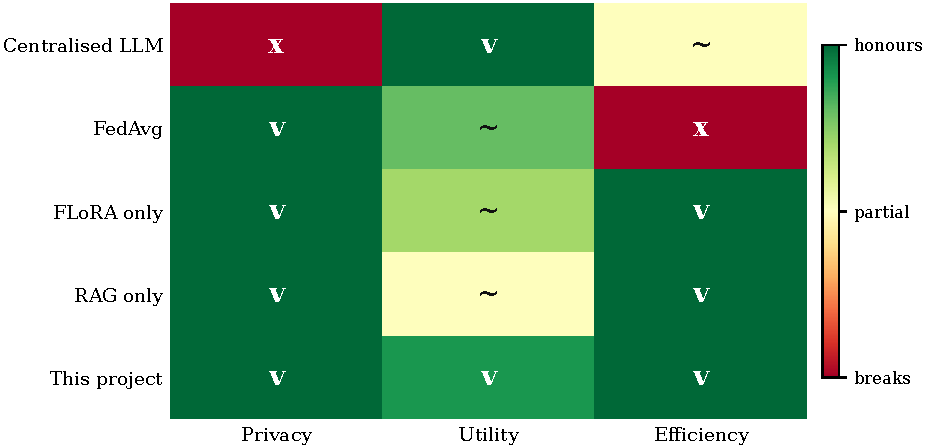
\includegraphics[width=0.92\linewidth]{res/fig-concept-gap-matrix.pdf}
    \caption[Gap in existing approaches]{Coverage of the three trilemma axes by existing approaches, motivating the present project's combined approach in Section~\ref{sec:meth:arch}. FedAvg~\cite{mcmahan2017communication} protects privacy and utility but is operationally inefficient at LLM scale. FLoRA alone~\cite{flora2024federated} solves efficiency and keeps utility but, without local retrieval, still requires bank-specific knowledge to live in the adapters. RAG alone externalises knowledge but does not itself perform federated training. This project combines the three and is the first row, to the best of current knowledge, that honours all three axes.}
    \label{fig:concept-gap-matrix}
\end{figure}

\section{Aim and Objectives}

\subsection{Aim}

This project designs, implements, and evaluates a privacy-first federated reasoning architecture, termed \textit{Thinking Inside the Box}, which resolves the Privacy-Utility-Efficiency Trilemma by decoupling reasoning (shared FLoRA adapters) from knowledge (per-node RAG over a local graph database). The architecture is domain-agnostic by design and is evaluated on the task of account-level AML classification using the IBM AML dataset \cite{weber2018scalablegraphlearningantimoney}.

\subsection{Objectives}

To meet this aim, the project pursues five SMART objectives.

\begin{enumerate}
    \setlength\itemsep{0em}
    \item \textbf{OI Architecture.} Implement a domain-agnostic federated LLM architecture with cleanly separated federation, retrieval, and model-adapter modules, using the Strategy design pattern to support interchangeable graph-store backends (Kuzu, NetworkX, Neo4j) without modifying the federation or RAG layers.
    \item \textbf{OII Simulation.} Construct a cross-silo simulation of three banking institutions using a lightweight in-process federated loop (informed by the Flower framework's client-strategy abstraction \cite{beutel2022flowerfriendlyfederatedlearning} but implemented natively to avoid the per-worker model-pickling overhead of Flower's Ray-based Virtual Client Engine on a single accelerator), with stratified 70/15/15 splits per node of the IBM AML dataset and non-identical data distributions that reflect real institutional heterogeneity.
    \item \textbf{OIII Benchmark.} Evaluate the proposed architecture against two baselines (centralised training and full-weight FedAvg) across six experimental conditions that cross three aggregators with two retrieval modes (flat versus RAG), over ten federation rounds.
    \item \textbf{OIV Trilemma measurement.} Quantify each condition on three axes: utility via F1 score~\cite{10.3115/1072064.1072067} on account-level AML labels, efficiency via total bytes transmitted per round and wall-clock latency, and privacy via Membership Inference Attack (MIA) AUC on exchanged adapter deltas, with the chance baseline at $0.5$.
    \item \textbf{OV Evidence.} Demonstrate, with reproducible data archived in the project repository, that the FLoRA-with-local-RAG configuration approaches the utility of centralised training while reducing communication volume by approximately three orders of magnitude and holding the MIA AUC close to the chance baseline.
\end{enumerate}

The project deliverables are a reproducible open-source codebase published at \url{https://github.com/SlaviXG/thinking-inside-the-box}, a benchmark dataset of per-round metrics for all six conditions, and this dissertation. All were delivered within the CSC3094 timeline, with the frozen benchmark run archived under git tag \texttt{benchmark-2026-04-02}.

\section{Dissertation Structure}

Chapter~\ref{ch:background} reviews the prior work that motivates and enables the proposed architecture, grouped into federated learning foundations, parameter-efficient fine-tuning, retrieval-augmented reasoning, and the AML task domain. Chapter~\ref{ch:method} describes the system architecture, implementation, testing strategy, and ethical considerations, including the novel bank-scoped pattern retriever that injects structural AML signals into the RAG context without crossing the privacy boundary. Chapter~\ref{ch:results} presents the six-condition benchmark, analyses the trilemma trade-offs along each axis, and discusses the evaluation's limitations. Chapter~\ref{ch:conclusions} summarises the achievements against the stated objectives and identifies concrete avenues for future work.


\chapter{Background Review}
\label{ch:background}

This chapter surveys the prior work that motivates and enables the \textit{Thinking Inside the Box} architecture. Each section concludes with an explicit statement of how the surveyed literature shapes a design choice in the present project.

\section{Federated Learning Foundations}
\label{sec:bg:fl}

Federated Learning was introduced by McMahan et al.~\cite{mcmahan2017communication} as Federated Averaging (FedAvg). Each client performs local stochastic gradient descent on its private partition, and the server aggregates updates by weighted mean. FedAvg transmits no raw records over the wire and, in the original paper, achieved competitive accuracy on MNIST and CIFAR-10 while reducing communication cost by one to two orders of magnitude relative to naive synchronous distributed SGD. Its theoretical convergence analysis relies on the assumption that client data distributions are not too far from identical (IID), an assumption that does not hold in cross-silo financial deployments. Subsequent work has documented accuracy degradation under heterogeneous non-IID settings and proposed variants such as FedProx and SCAFFOLD to address client drift. For this dissertation, however, the principal limitation of FedAvg is elsewhere: its communication cost scales linearly with the number of trainable parameters, which for an 8-billion-parameter reasoning backbone amounts to roughly 16~GB per client per round in fp16 precision (and approximately 32~GB once the server-to-client broadcast is included), as Figure~\ref{fig:concept-flora-vs-fedavg} compares against the FLoRA payload introduced later in the chapter. This makes full-weight FedAvg operationally infeasible at modern LLM scale.

The experimental substrate adopted for this project is a bespoke in-process federated simulation loop whose client interface (\texttt{fit}, \texttt{evaluate}, \texttt{get\_parameters}, \texttt{set\_parameters}) is modelled on the Flower framework~\cite{beutel2022flowerfriendlyfederatedlearning}. Flower's own Virtual Client Engine was evaluated and rejected: it schedules each client on a separate Ray worker process, and each worker pickles its own copy of the 8-billion-parameter backbone alongside the activations, gradient-checkpointing buffers, AdamW optimiser state, and KV cache that one fine-tuning round needs. Although the quantised backbone occupies only approximately 6~GB at 4-bit NF4~\cite{nvidia2018t4, bisong2019google}, three concurrent workers compound this footprint - each with its own copy of the backbone and a full set of per-worker fine-tuning buffers - past the 40~GB available on the Colab A100, triggering OOM despite the on-disk footprint being well within budget. The custom loop instead runs all clients sequentially in the main process, loading the base model once and sharing it by reference. This is essential for a simulation-first methodology on a single accelerator. The chief limitation of a simulation-only evaluation is that it does not capture real network latency, packet loss, or straggler behaviour. This project partially addresses the limitation by reporting wall-clock latency separately for the fit, evaluation, and aggregation stages.

\begin{figure}[t]
    \centering
    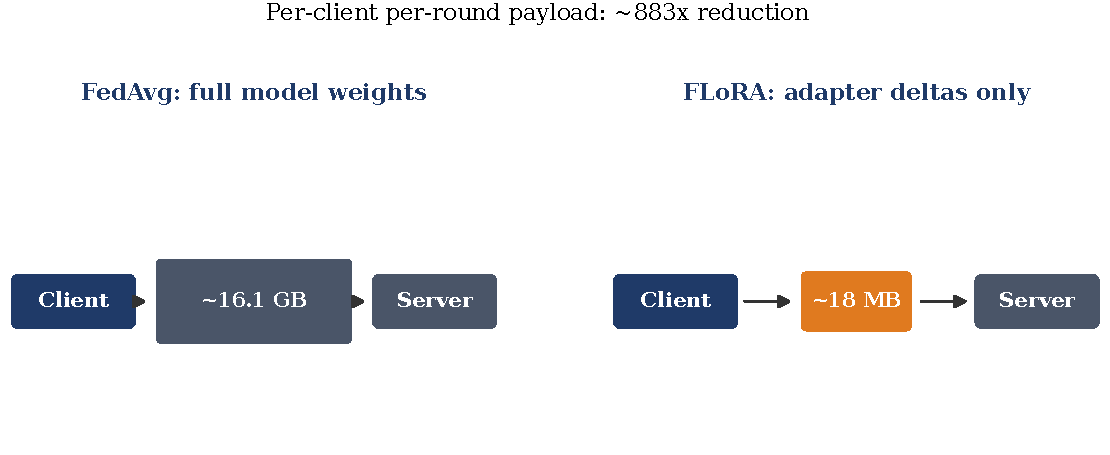
\includegraphics[width=0.85\linewidth]{res/fig-concept-flora-vs-fedavg.pdf}
    \caption[FLoRA vs FedAvg communication footprint]{Per-round communication footprint, supporting the parameter-efficient fine-tuning argument in Section~\ref{sec:bg:peft} and the production-deployment recasting in Section~\ref{sec:meth:production}. Classical FedAvg~\cite{mcmahan2017communication} transmits the full 8-billion-parameter backbone, approximately 16~GB per client per round at fp16 precision. FLoRA~\cite{flora2024federated} transmits only low-rank adapter deltas ($r=8$, \texttt{q\_proj}+\texttt{v\_proj}), approximately 18~MB per client per round including the Fernet authenticated-encryption wrapper - a reduction of nearly three orders of magnitude (approximately 880x) at the same backbone scale.}
    \label{fig:concept-flora-vs-fedavg}
\end{figure}

Two conclusions follow. First, FedAvg remains the reference baseline against which any federated method must be compared, and for this reason it is one of the two baselines in the six-condition benchmark of Chapter~\ref{ch:results}. Second, FedAvg's communication cost, illustrated in Figure~\ref{fig:concept-flora-vs-fedavg}, is the concrete problem that motivates the parameter-efficient alternatives surveyed in Section~\ref{sec:bg:peft}.

\section{The Privacy-Utility-Efficiency Trilemma}
\label{sec:bg:trilemma}

The tension between the three axes of privacy, utility, and efficiency has been formalised in two complementary strands of work. Zhou et al.~\cite{plosone2023e0338822} propose DualMask, a framework that optimises the joint privacy-utility-efficiency objective through orthogonal gradient perturbation and reinforcement-learning-guided particle swarm optimisation. Their principal contribution is a quantitative accounting of how strengthening the privacy axis, for example by injecting differential privacy noise, predictably degrades utility at a measurable rate. DualMask is a parameter-tuning approach: it assumes a fixed architecture and searches the trade-off surface. Its limitation, from the perspective of the present project, is that it accepts the trilemma as axiomatic and optimises within it, rather than attempting to restructure the architecture so that the three axes no longer compete.

Allouah et al.~\cite{allouah2023trilemma} address a closely related privacy-robustness-utility trilemma and prove impossibility bounds for distributed learning under adversarial assumptions. Their theoretical result establishes that no single algorithm can simultaneously achieve optimality on all three axes when adversaries are free to submit arbitrary updates. This framing is less directly relevant here, because the cross-silo financial setting modelled in this project assumes honest-but-curious participants rather than active adversaries; the impossibility bounds therefore do not directly apply. However, the work is important for demonstrating that even under relaxed adversarial assumptions, the axes remain provably in tension when they are defined over the same learnable parameters.

The conclusion drawn here is architectural rather than algorithmic. The trilemma, as usually formulated, treats the three axes as intrinsic properties of a federated learning system. This dissertation adopts a different position: the trilemma is a property of the specific decision to co-locate reasoning capacity and sensitive knowledge in the same learnable parameters. Once those two concerns are \textit{separated}, the three axes cease to compete directly. Shared FLoRA adapters carry the reasoning update and are communicated cheaply; local RAG indices carry the sensitive knowledge and never leave the node. This separation is what the techniques reviewed in Sections~\ref{sec:bg:peft} and~\ref{sec:bg:rag} make technically feasible.

\section{Parameter-Efficient Fine-Tuning}
\label{sec:bg:peft}

Low-Rank Adaptation (LoRA), introduced by Hu et al.~\cite{hu2021lora}, observes that pretrained language model updates during fine-tuning tend to lie on a low-rank manifold, and approximates the weight delta $\Delta W$ as the product $BA$ of two low-rank matrices. With the base model frozen and only $B$ and $A$ trainable, the number of learnable parameters drops by three or more orders of magnitude relative to full fine-tuning, with negligible loss of downstream task performance on typical benchmarks. LoRA is the empirical basis of parameter-efficient fine-tuning for modern large language models. Its limitations are that the rank $r$ must be chosen in advance and that the approach is not, in its original form, designed for federated aggregation.

Dettmers et al.~\cite{dettmers2024qlora} extend LoRA with 4-bit quantised storage of the frozen base model (QLoRA). Quantisation reduces the base model's memory footprint by approximately a factor of four, which is what permits an 8-billion-parameter backbone to fit within the 16~GB of VRAM available on consumer-grade accelerators such as the NVIDIA T4~\cite{nvidia2018t4}. The limitation of 4-bit quantisation is that numerical errors are introduced at every forward pass; in practice QLoRA compensates with blockwise double quantisation and a custom normal-float data type, but the technique remains sensitive to the choice of block size and is known to accumulate error in very long-horizon fine-tuning runs.

Wang et al.~\cite{flora2024federated} propose FLoRA, a federated extension of LoRA that specifically addresses aggregation in the presence of heterogeneous adapter ranks across clients. FLoRA stacks client adapters and applies singular value decomposition to recover a low-rank server-side update. This matters because in a real cross-silo deployment different clients may afford different adapter ranks, and naive parameter-wise averaging of LoRA matrices is mathematically incorrect when ranks differ: the matrix product $BA$ does not distribute over element-wise averaging in the factor matrices. FLoRA's practical limitation is that the stacking-plus-SVD operation incurs a server-side cost that grows with the aggregate rank across clients.

The conclusion from this body of work is that FLoRA is the appropriate federation primitive for this project. It delivers approximately a nine-hundred-fold reduction in communication payload relative to full-weight FedAvg on the 8B backbone (18~MB per client per round, versus roughly 16~GB at fp16 precision), it handles rank heterogeneity, and it composes cleanly with QLoRA for GPU-memory efficiency. FLoRA is consequently the federated aggregator of interest in the benchmark of Chapter~\ref{ch:results}.

\section{Retrieval-Augmented Generation}
\label{sec:bg:rag}

Lewis et al.~\cite{lewis2021retrievalaugmentedgenerationknowledgeintensivenlp} introduced Retrieval-Augmented Generation (RAG) as a method for knowledge-intensive natural language processing tasks. A RAG system pairs a dense retrieval component with a sequence-to-sequence generator: at inference time the retriever returns the top-$k$ passages relevant to the input, and the generator conditions its output on both the query and the retrieved context. The principal practical consequence is that the system's factual knowledge can be updated by updating the retrieval index, without retraining the generator. The primary limitation of the original RAG formulation, from the perspective of this project, is that it assumes a single, globally shared retrieval index. This is incompatible with a federated setting in which each node's knowledge base must remain private.

The insight that this project brings to bear on that limitation is that the RAG paradigm generalises naturally to a federation of \textit{local} retrieval indices, provided that the retrieval context is assembled entirely on the client side and is never shipped to the server. Under this constraint, the RAG index inherits the privacy guarantees of the node that owns it, and only the generator's reasoning capability participates in the federation. In the AML setting specifically, the retrieval context is derived from a per-node graph database: transactions, accounts, and their relational structure. Graph-based retrieval is essential for AML because money laundering typologies are defined by multi-hop structural signals such as structuring, layering, pass-through chains, and fan-out bursts, which a flat text retriever cannot detect by similarity matching alone. The present project contributes a bank-scoped pattern detector that translates structural graph queries into named, LLM-digestible signals without crossing the privacy boundary; the detailed design is presented in Chapter~\ref{ch:method}.

The conclusion is that RAG provides the architectural pattern for externalising knowledge from model weights, and that the pattern can be lifted to the federated setting by keeping the retrieval index strictly on-node. This is the second half of the decoupling strategy motivated in Section~\ref{sec:bg:trilemma}, illustrated in Figure~\ref{fig:concept-rag-vs-parametric}.

\begin{figure}[t]
    \centering
    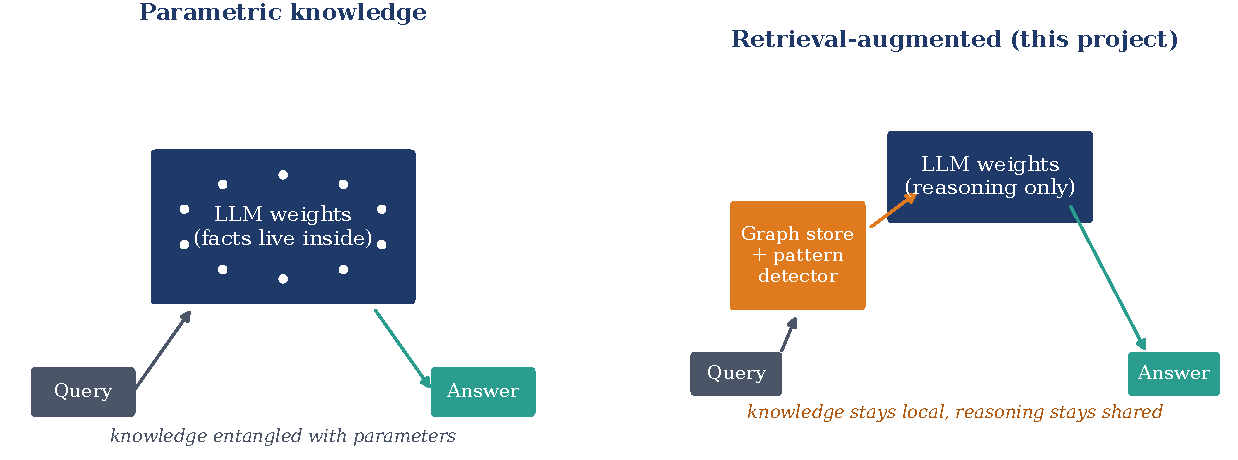
\includegraphics[width=0.92\linewidth]{res/fig-concept-rag-vs-parametric.pdf}
    \caption[Parametric knowledge vs RAG]{Parametric versus retrieval-augmented knowledge, supporting the decoupling argument that drives the design in Section~\ref{sec:meth:arch}. Left: a parametric model stores what it knows inside its trainable weights, so updating knowledge and updating reasoning are the same operation. Right: RAG externalises the knowledge into a retrievable store and lets the model read from it at inference time, so knowledge can stay local and private while the reasoning component is trained across institutions.}
    \label{fig:concept-rag-vs-parametric}
\end{figure}

\section{Reasoning Language Models and the AML Task Domain}
\label{sec:bg:reasoning}

The backbone model used in this project is the DeepSeek-R1-Distill-Llama-8B variant of the DeepSeek-R1 family~\cite{deepseek2025r1}. DeepSeek-R1 is a reasoning-oriented LLM trained with reinforcement learning against verifiable rewards, and it exhibits emergent chain-of-thought behaviour on quantitative and symbolic tasks. The distilled 8B variant is approximately $84\times$ smaller than the full R1 model ($8.03$~billion parameters versus $671$~billion in the Mixture-of-Experts base) while retaining the reasoning prompt format, which makes it tractable on a single consumer-grade accelerator at 4-bit precision. The relevant limitation, from a federation standpoint, is that such a model is large by the standards of classical federated learning; this is precisely what motivates the QLoRA-plus-FLoRA stack adopted in this project.

For the AML task itself, the IBM AML dataset of Weber et al.~\cite{weber2018scalablegraphlearningantimoney} provides a synthetic yet structurally realistic corpus of interbank transactions, partitioned by originating bank and annotated with account-level laundering labels. The synthetic provenance is both a strength and a limitation: it sidesteps the regulatory hurdles that would accompany real banking data and enables open, reproducible research, but it does not fully capture the adversarial creativity of real-world money launderers, whose strategies evolve to evade detection. The dataset's account-level labels align with the F1 score as the natural utility metric, following the evaluation tradition formalised in the MUC series~\cite{10.3115/1072064.1072067}.

The conclusion of this section is that DeepSeek-R1-Distill-8B supplies a reasoning-capable backbone appropriate for the chain-of-thought investigative style required by AML triage, and the IBM AML dataset supplies a domain-appropriate, openly available benchmark. Together they satisfy the task-level requirements of the architecture whose design is detailed in the next chapter.


\chapter{Methodology}
\label{ch:method}

\section*{Reader's orientation}

This chapter is written for a reader with general computer-science background and does not assume prior exposure to financial regulation, money-laundering investigation, or banking operations. Three terms reappear throughout and are worth fixing here so that they do not impede the rest of the chapter.

\textit{Cross-silo Federated Learning} is the variant of FL in which a small number of well-identified, contractually bound institutions (banks, hospitals, law firms) each hold a partition of the data and want to learn a shared model without exchanging records. It is distinct from \textit{cross-device} FL, where the participants are millions of unidentified end-user devices (smartphones, browsers). The cross-silo setting is the right model for this dissertation because the AML deployment scenario has a few participants, all known to one another, all with substantial compute, and all under the same class of regulation. Cross-silo participants are usually assumed to follow the protocol; cross-device participants are usually assumed to be unreliable and possibly adversarial.

\textit{Anti-Money Laundering (AML)} is the regulatory and analytic discipline by which financial institutions detect and report transactions consistent with money laundering or terrorist financing. From a computer-science angle the core task is binary classification on graph-structured data: each account is labelled \textit{clean} or \textit{suspicious}, and the analytic signal sits in the multi-hop transaction structure rather than in any individual transaction. Real banks file \textit{Suspicious Transaction Reports} (STRs) under FATF Recommendation~20 and its national transpositions; the dissertation treats STR generation as a downstream consequence of correctly classifying suspicious accounts.

\textit{The privacy boundary} is the architectural construct that names which artefacts may leave a bank node and which may not. In the design that follows, raw transactions, account identifiers, graph queries, and any statistic computed over raw transactions remain inside the boundary. The only artefact that crosses it is an encrypted low-rank adapter weight delta. The boundary is enforced not by policy but by code structure: the modules with raw-data access do not appear in the federated communication path. This idea is doing the heavy lifting in the regulatory framing later in the chapter.

The chapter then proceeds as follows. Section~\ref{sec:meth:requirements} formalises the requirements derived from the objectives stated in Chapter~\ref{ch:introduction}. Section~\ref{sec:meth:regulatory} maps the architecture to the regulatory regimes under which it would be deployed in the AML case study, and identifies which design decision satisfies which regulation. Section~\ref{sec:meth:arch} presents the system architecture and the design decisions that make it domain-agnostic. Section~\ref{sec:meth:impl} gives a component-by-component account of the implementation. Section~\ref{sec:meth:production} translates the benchmark numbers into deployment-time figures (WAN bandwidth, GPU-hour cost, audit artefacts). Section~\ref{sec:meth:testing} describes the testing and reproducibility strategy. Section~\ref{sec:meth:threat} states the threat model under which the privacy claims hold. Section~\ref{sec:meth:ethics} reports on ethical considerations. Section~\ref{sec:meth:deviations} documents deviations from the project proposal and the reasoning behind each.

\section{Requirements}
\label{sec:meth:requirements}

The requirements below were derived directly from the five SMART objectives stated in Section~\ref{ch:introduction}. Functional requirements describe what the system must do; non-functional requirements constrain how it must behave within the resources available to an undergraduate dissertation.

\subsection{Functional requirements}

\begin{itemize}
    \setlength\itemsep{0em}
    \item \textbf{F1 Domain agnosticism.} The core pipeline must make no assumptions about the underlying data domain or task. Moving from the AML case study to a different regulated domain (for example, healthcare) must require changes only to the ingestion layer and the retrieval-time prompt, not to the federation or adapter-training layers.
    \item \textbf{F2 Pluggable graph backends.} The local knowledge store must be interchangeable between at least three implementations (an embedded store suitable for simulation, an in-memory store suitable for unit tests, and a server-backed store suitable for real distributed deployment), without requiring changes to the federation or RAG layers.
    \item \textbf{F3 Federated training.} The system must train a single reasoning adapter across at least three simulated bank nodes, exchanging only low-rank adapter deltas with a central server.
    \item \textbf{F4 Baseline comparability.} The system must support three aggregators (centralised, FedAvg, FLoRA) and two retrieval modes (flat, RAG) so that a $3 \times 2$ benchmark can be run from a single codebase.
    \item \textbf{F5 Trilemma measurement.} The system must report, per federation round and per client, the F1 score (utility), the number of bytes transmitted (efficiency), and a Membership Inference Attack AUC (privacy).
    \item \textbf{F6 Reproducibility.} Every benchmark run must emit a configuration file and a history file that together are sufficient to reconstruct the reported numbers from the archived code state.
\end{itemize}

\subsection{Non-functional requirements}

\begin{itemize}
    \setlength\itemsep{0em}
    \item \textbf{N1 Single-GPU simulation.} The entire benchmark must run on a single Google Colab A100 instance, which bounds peak GPU memory and run time.
    \item \textbf{N2 Privacy boundary preservation.} No raw transaction record, nor any statistic aggregated over raw records, must cross the client-server boundary. Only adapter deltas, cryptographically protected in transit, may leave a node.
    \item \textbf{N3 Strong typing of configuration.} All experimental parameters (ranks, learning rates, retrieval modes, sample budgets) must live in a single dataclass so that runs are fully parameterised and reproducible.
    \item \textbf{N4 Operational observability.} The pipeline must emit per-client, per-round logs for fit loss, evaluation metrics, and MIA AUC, allowing retrospective diagnosis of convergence issues.
    \item \textbf{N5 Separation of concerns.} Federation logic, RAG pipeline, and model adapter code must live in distinct modules with minimal coupling, so that each can be modified or replaced without affecting the others.
\end{itemize}

\section{Regulatory Framing}
\label{sec:meth:regulatory}

The architecture is presented in this dissertation under the AML case study, but the regulatory regimes against which it is justified here apply, with appropriate substitution of the sector-specific instruments, to any domain in which a federation of institutions must collaborate on inference without pooling raw records: cross-hospital clinical research under HIPAA or its national equivalents, inter-firm legal-discovery pipelines, and cross-jurisdiction tax compliance among them. The architecture is therefore not specialised to any one regime. The following five subsections name the five regulatory regimes most directly relevant to the AML deployment case, and tie each to a specific design decision elsewhere in this chapter.

\subsection{Data protection by design (GDPR Article 25; data minimisation under Article 5(1)(c))}

Article 25 of the General Data Protection Regulation~\cite{gdpr2016} requires controllers to implement, at the time the means of processing are determined, technical and organisational measures designed to integrate data-protection principles into the processing itself. Article 25(2) further requires that, by default, only personal data necessary for each specific purpose are processed, and that this default applies to ``the amount of personal data collected, the extent of their processing, the period of their storage and their accessibility''. Article 5(1)(c) names data minimisation as one of the six principles that Article 25 is required to implement: data must be ``adequate, relevant and limited to what is necessary in relation to the purposes for which they are processed''.

The privacy boundary defined in Section~\ref{sec:meth:arch} and visualised in Figure~\ref{fig:concept-privacy-boundary} is the architectural mechanism by which both Articles are satisfied at design time rather than at policy time. No code path in the federation, retrieval, or model layers exposes raw transactions outside the bank node that owns them; the only artefact crossing the boundary is the encrypted low-rank adapter delta. The default is therefore not ``share, with policy controls'' but ``do not share, by construction'', which is what Article 25(2) calls for.

\subsection{Suspicious transaction reporting and record-keeping (FATF Recommendations 10, 11, 20; UK MLR 2017)}

The Financial Action Task Force's 40 Recommendations~\cite{fatf2025recommendations} are the international standard for AML and counter-terrorist-financing controls. Three are directly relevant here. Recommendation~10 obliges financial institutions to perform customer due diligence; Recommendation~11 obliges them to retain transaction and CDD records for at least five years; Recommendation~20 obliges them to file suspicious transaction reports with the national financial intelligence unit. In the United Kingdom these obligations are transposed by the Money Laundering, Terrorist Financing and Transfer of Funds (Information on the Payer) Regulations 2017~\cite{ukmlr2017}, whose Regulations~27-32 codify CDD and whose Regulation~40 codifies record-keeping at up to ten years.

The bank-scoped pattern detector of Section~\ref{sec:meth:impl:patterns} is the architectural component that supports STR generation under Recommendation~20: each detected typology (pass-through, structuring, fan-out, rapid-burst, intra-bank cycle) is exactly the kind of structural signal that an FIU expects to see substantiating an STR. The detector's confinement to a single bank's partition is what keeps the support evidence within Regulation~40's record-keeping perimeter and avoids cross-institution data flows that would themselves require a separate legal basis.

\subsection{Cross-institution information sharing (USA PATRIOT Act \texorpdfstring{\S}{Section}~314(b))}

Section~314(b) of the USA PATRIOT Act provides a statutory safe harbour permitting US financial institutions to share information with one another for the purpose of identifying and reporting suspected money laundering or terrorist financing activities~\cite{fincen314b}. The safe harbour is voluntary and requires the participating institution to file a notice with FinCEN; once filed, it provides protection against most privacy-related civil liabilities arising from the sharing.

The federated architecture provides the analytic value that motivates a \S~314(b) sharing arrangement (cross-institution detection of typologies that are deliberately fragmented across the interbank payment system) without requiring the sharing of raw records that the safe harbour permits but that institutions remain reluctant to execute in practice. Only the encrypted adapter delta, an arbitrary learned transformation of each bank's local supervisory signal, crosses the boundary toward the aggregator. This is consistent with \S~314(b)'s purpose, but operates at a strictly stronger privacy posture than the underlying statute requires.

\subsection{Model risk management (PRA SS1/23 in the UK; OSFI Guideline E-23 in Canada)}

The Prudential Regulation Authority's Supervisory Statement SS1/23~\cite{prass123}, in force since 17~May 2024, sets out five principles for model risk management at UK-incorporated banks, building societies, and PRA-designated investment firms. The Office of the Superintendent of Financial Institutions Canada finalised Guideline E-23~\cite{osfie23} on 11~September 2025, and the Guideline takes effect for all federally regulated financial institutions on 1~May 2027 with explicit AI/ML scope. Both regimes converge on the same expectations: the model lifecycle must be auditable, the inputs and decisions must be reproducible, and the institution must maintain documented controls over training, validation, and deployment.

The reproducibility apparatus of this dissertation operationalises those expectations directly. Per-run configuration is serialised to a single \texttt{Config} dataclass (Section~\ref{sec:meth:impl}); per-round metrics are appended to history JSON files; the code state that produced each archived benchmark is pinned by an annotated git tag (\texttt{benchmark-2026-04-02}, commit \texttt{01a6cce}). The same artefact set reconstructs both the inputs and the decisions of every reported experiment, which is what an SS1/23 or E-23 audit asks for.

\subsection{Criminal-law severity (Sixth Anti-Money Laundering Directive)}

Directive (EU) 2018/1673, the Sixth Anti-Money Laundering Directive~\cite{eu6amld2018}, raises the EU minimum prison sentence for money laundering to four years, lists 22 predicate offences that all member states must criminalise, and extends criminal liability to legal persons. The Directive entered into force on 3~December 2020, with transposition required by 3~June 2021.

The bearing of 6AMLD on this dissertation is asymmetric loss: the cost of a false negative (a missed launderer that the bank could have detected) is not a model-accuracy concern but a corporate criminal liability concern, because the bank itself becomes a legal person liable under the Directive's corporate-liability provisions. This asymmetry is the regulatory backdrop against which the cost-of-misclassification analysis in Section~\ref{sec:results:cost} is reported, and it explains why the dissertation reports both peak and final-round F1: the operational acceptance condition is dominated by recall on the laundering class, not by an aggregate metric.

\subsection{Compliance summary}
\label{sec:meth:regulatory:summary}

Table~\ref{tab:regulatory-compliance} summarises the relationship between each regulatory regime named above and the architectural mechanism that addresses it. The compliance column distinguishes three honest cases: \textbf{Met by design} means a regulation's required default is realised in code, not in policy; \textbf{operationally supported} means the architecture produces the artefacts the regulation expects (audit trails, STR-shaped signals, retention-friendly records) without itself being the operational system that satisfies the obligation end-to-end; \textbf{out of scope} means the obligation falls on a layer of the institution's stack that this dissertation does not implement. The dissertation does not claim formal regulatory certification; the assessment in the table is the author's mapping of design decisions to obligations and would be the starting point for a real legal review at deployment time.

\begin{table}[H]
\centering
\caption[Regulation x architectural mechanism compliance]{Regulation x architectural mechanism compliance summary, supporting Sections~\ref{sec:meth:regulatory} and~\ref{sec:meth:arch}. ``Met by design'' obligations are enforced in code; ``operationally supported'' obligations have the necessary audit or signal artefacts but require an institution-side process to discharge end-to-end; ``out of scope'' obligations fall on layers the dissertation does not implement.}
\label{tab:regulatory-compliance}
\small
\begin{tabularx}{\textwidth}{p{3.2cm} p{4.0cm} X p{2.4cm}}
\toprule
\textbf{Regulation} & \textbf{Obligation} & \textbf{Architectural mechanism} & \textbf{Status} \\
\midrule
GDPR Art.~5(1)(c)~\cite{gdpr2016} & Data minimisation: process only personal data necessary for the purpose & Privacy boundary: only encrypted adapter deltas leave a node; raw transactions and account identifiers never traverse the federation path & Met by design \\
\addlinespace
GDPR Art.~25~\cite{gdpr2016} & Data protection by design and by default: technical measures integrating data-protection principles into processing itself & Module layout segregates raw-data access (\texttt{src/data/}, \texttt{src/graph/}) from the federation path (\texttt{src/federation/}); the default is non-disclosure & Met by design \\
\addlinespace
GDPR Art.~22~\cite{gdpr2016} & Right not to be subject to a decision based solely on automated processing & Verdict-first target format positions the LLM output as triage input to a human investigator; STR generation remains a human decision & Architecturally aligned (out of scope as a runtime guarantee) \\
\addlinespace
FATF Rec.~10~\cite{fatf2025recommendations} & Customer due diligence at onboarding & CDD is performed at customer onboarding, before transactions reach the model & Out of scope \\
\addlinespace
FATF Rec.~11~\cite{fatf2025recommendations}; UK MLR 2017 Reg.~40~\cite{ukmlr2017} & Record-keeping (FATF: 5 years; UK: up to 10 years) & Per-round JSON history files plus pinned git tag give a reproducible record of inputs, model state, and per-account decisions, and integrate cleanly into a longer-retention archival store & Operationally supported \\
\addlinespace
FATF Rec.~20~\cite{fatf2025recommendations} & Suspicious transaction reporting to FIU & Bank-scoped pattern detector emits named typologies (pass-through, structuring, fan-out, rapid-burst, intra-bank cycle) suitable as STR support evidence & Operationally supported \\
\addlinespace
USA PATRIOT \S~314(b)~\cite{fincen314b} & Voluntary information-sharing safe harbour for AML purposes & Federation produces the cross-institution analytic value at a privacy posture stricter than the statute requires; only encrypted deltas, never records, traverse the boundary & Architecturally consistent (stricter than required) \\
\addlinespace
PRA SS1/23~\cite{prass123} & Auditable model lifecycle, five MRM principles, in force 17 May 2024 & Config dataclass + history JSON + annotated git tag form a reproducible inputs/outputs/code triple sufficient for the audit trail & Operationally supported \\
\addlinespace
OSFI Guideline E-23~\cite{osfie23} & Auditable AI/ML model lifecycle for FRFIs, effective 1 May 2027 & Same artefact triple as SS1/23; the architecture does not need to change to comply with E-23's AI/ML scope & Operationally supported \\
\addlinespace
6AMLD~\cite{eu6amld2018} & 4-year minimum sentence; corporate criminal liability; 22 predicate offences & Asymmetric-loss framing throughout: peak and final F1 score reported separately, recall-driven cost analysis in Section~\ref{sec:results:cost}, MIA limits acknowledged & Acknowledged (regulatory backdrop) \\
\bottomrule
\end{tabularx}
\end{table}

The architecture therefore complies, by design, with the data-protection regimes that govern what may leave a participating institution; it operationally supports the AML record-keeping and STR regimes, and the UK and Canadian model-risk regimes, in the sense that it produces the artefacts those regimes expect; it sits within (and stricter than) the US information-sharing safe harbour without depending on it. Two obligation classes remain explicitly out of scope: customer due diligence at onboarding and end-to-end automated-decision compliance, both of which belong to layers of the institution's stack that this dissertation does not implement.

\section{System Architecture}
\label{sec:meth:arch}

\subsection{Design principle: decoupling reasoning from knowledge}

The architectural premise of the project, motivated in Sections~\ref{sec:bg:trilemma} and~\ref{sec:bg:rag}, is that the Privacy-Utility-Efficiency Trilemma is not intrinsic to federated LLMs. It is a consequence of a specific design decision, namely, co-locating reasoning capacity and sensitive knowledge within the same learnable parameters. Once those two concerns are separated into distinct system components, the three axes cease to compete directly:

\begin{itemize}
    \setlength\itemsep{0em}
    \item \textbf{Reasoning} lives in the shared FLoRA adapters. These are small (megabytes, not gigabytes), they carry no raw data, and they are the only artefact that traverses the network.
    \item \textbf{Knowledge} lives in a per-node local RAG index, implemented over a graph database that holds the node's private transactions. The index is queried only by the local client at inference time, and the retrieved context is used only as prompt material for the frozen base model.
\end{itemize}

This decoupling is the central contribution of the architecture, and it dictates the module layout described below. Figure~\ref{fig:concept-privacy-boundary} visualises the resulting privacy boundary: raw transactions, the graph store, the local adapter, and the pattern detector all live inside each bank's dashed orange perimeter, while the only artefact crossing the perimeter is the encrypted adapter delta.

\begin{figure}[t]
    \centering
    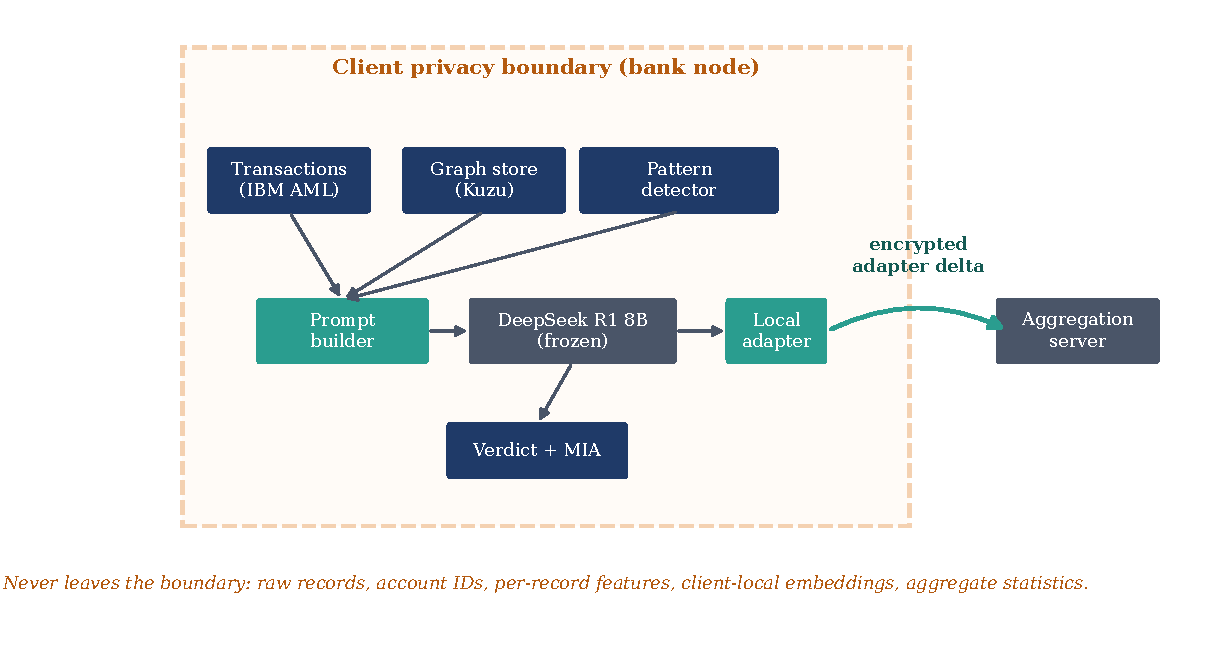
\includegraphics[width=0.88\linewidth]{res/fig-concept-privacy-boundary.pdf}
    \caption[Privacy boundary around one bank node]{Privacy boundary around one bank node, supporting Section~\ref{sec:meth:arch} (design principle) and Section~\ref{sec:meth:regulatory} (GDPR Articles 5(1)(c) and 25). Transactions, the local graph store, the pattern detector, the frozen backbone plus adapter, and the generated verdict all remain inside the orange dashed boundary. Only the encrypted adapter delta crosses the boundary toward the aggregation server. Raw records, account identifiers, and any statistic aggregated over raw records never leave the node.}
    \label{fig:concept-privacy-boundary}
\end{figure}

\subsection{Module layout}

The Python package \texttt{src/} is organised into six top-level modules, each with a single responsibility.

\begin{itemize}
    \setlength\itemsep{0em}
    \item \texttt{src/data/} ingests the IBM AML CSV, partitions it by originating bank, and produces stratified 70/15/15 train/validation/test splits per partition.
    \item \texttt{src/graph/} contains the \texttt{GraphStore} abstract interface, three concrete backends (Kuzu, NetworkX, Neo4j), a factory, and the bank-scoped pattern detection module.
    \item \texttt{src/model/} loads the DeepSeek-R1-Distill-Llama-8B backbone under 4-bit QLoRA quantisation and attaches the LoRA adapter.
    \item \texttt{src/pipeline/} assembles the prompt for a target account, runs greedy generation against the adapted model, and parses the verdict from the model's reply.
    \item \texttt{src/federation/} contains the in-process federated client (fit, evaluate, MIA, with a Flower-compatible interface), the aggregation strategies (FLoRA and FedAvg), and the centralised baseline runner.
    \item \texttt{src/security/} implements the symmetric encryption wrapper used to protect adapter deltas in transit.
\end{itemize}

The federation layer depends only on abstract interfaces from the graph and pipeline layers; it has no awareness of which concrete graph backend is in use, nor of the specifics of AML pattern detection. This satisfies F1 (domain agnosticism) and N5 (separation of concerns). The end-to-end system is shown in Figure~\ref{fig:arch-system}.

\begin{figure}[t]
    \centering
    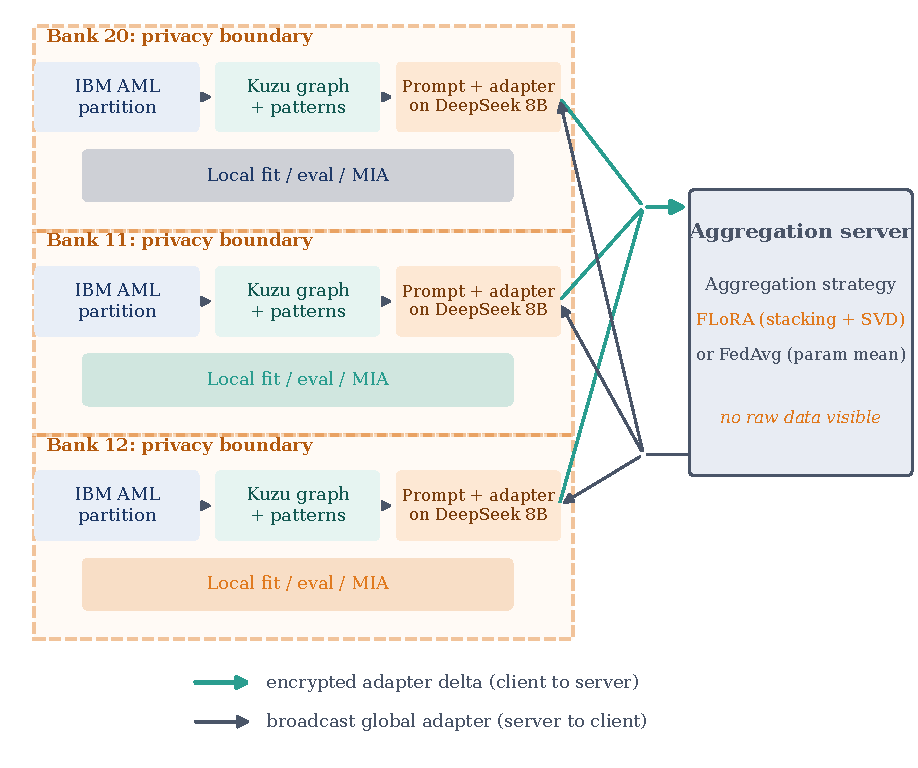
\includegraphics[width=0.96\linewidth]{res/fig-arch-system.pdf}
    \caption[Federated system architecture]{Federated system architecture, supporting Section~\ref{sec:meth:arch} (module layout). Three banks (left) each run an identical local pipeline: ingestion from the IBM AML partition, a Kuzu graph store, bank-scoped pattern detection, prompt construction, and a DeepSeek-R1-Distill-Llama-8B backbone with a QLoRA-quantised FLoRA adapter. Only encrypted adapter deltas (teal) cross the orange privacy boundary toward the aggregation server (right), which applies the configured strategy (FLoRA stacking + SVD, or FedAvg) without ever observing raw records.}
    \label{fig:arch-system}
\end{figure}

\subsection{Strategy pattern for graph stores}
\label{sec:meth:strategy}

The graph layer is the most substantial design decision in the project. It uses the Strategy pattern~\cite{gof1994} to achieve F2 (pluggable backends), and it is intentionally the only place in the codebase where a concrete database technology is named: every other layer talks to the abstract \texttt{GraphStore} interface, so swapping the backend is a localised change.

\texttt{src/graph/base.py} defines an abstract \texttt{GraphStore} interface with four operations: \texttt{ingest(transactions)}, \texttt{retrieve\_context(account\_id, mode)}, \texttt{structural\_signals(account\_id)}, and \texttt{close()}. Three concrete classes implement this interface:

\begin{itemize}
    \setlength\itemsep{0em}
    \item \texttt{KuzuGraphStore} is the default. Kuzu is an embedded graph database that stores one \texttt{.db} file per bank node, with negligible memory overhead and no server to manage. This makes it ideal for the simulation-first development path.
    \item \texttt{NetworkXGraphStore} is a purely in-memory backend used for unit testing the pattern detectors against hand-constructed transaction graphs. It is intentionally slow and unoptimised; its role is to have predictable semantics for test assertions.
    \item \texttt{Neo4jGraphStore} is provided for real distributed deployments where multiple processes on one node might share a single graph store, or where Cypher-based external tooling is desired.
\end{itemize}

A factory function in \texttt{src/graph/factory.py} selects the concrete backend based on a single \texttt{Config.graph\_backend} string. The federation and RAG layers depend only on the abstract interface; they will continue to work if a new backend (for example, TigerGraph or ArangoDB) is added later. Figure~\ref{fig:arch-strategy-pattern} shows the resulting class structure. This is exactly the kind of structural adaptability called for by the project instruction that the architecture must be reusable in practice beyond the dissertation.

\begin{figure}[t]
    \centering
    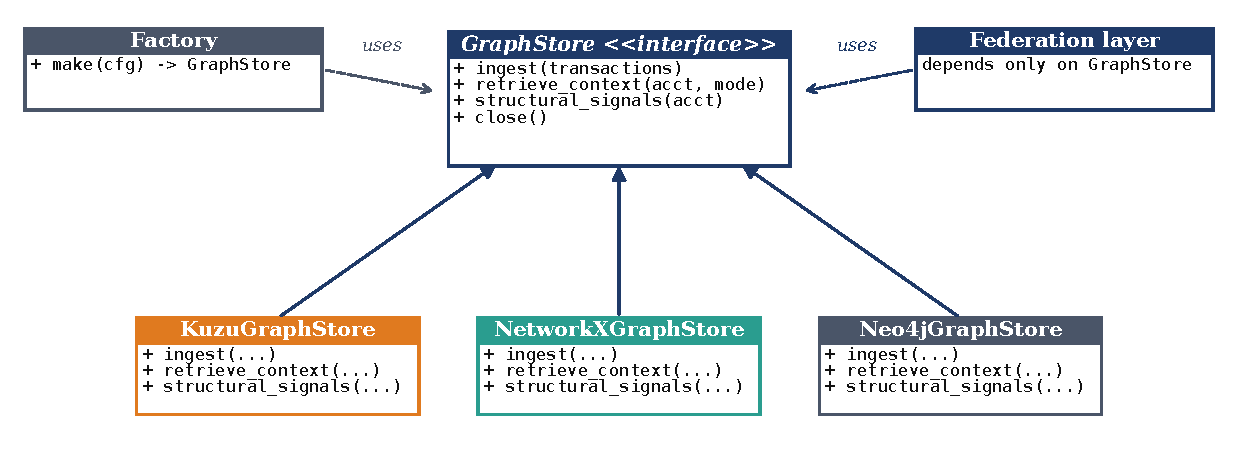
\includegraphics[width=0.82\linewidth]{res/fig-arch-strategy-pattern.pdf}
    \caption[Strategy pattern for graph backends]{Strategy pattern for pluggable graph backends, supporting Section~\ref{sec:meth:strategy}. The \texttt{GraphStore} abstract base class declares the four operations that the federation and RAG layers depend on. Three concrete implementations (\texttt{KuzuGraphStore}, \texttt{NetworkXGraphStore}, \texttt{Neo4jGraphStore}) satisfy the interface; a factory selects the concrete backend at runtime from the \texttt{Config.graph\_backend} string. Higher layers never import a concrete class, which satisfies F2 (pluggable backends).}
    \label{fig:arch-strategy-pattern}
\end{figure}

\subsection{Data and control flow in one federation round}

A single federation round proceeds as follows, and the benchmark consists of ten such rounds repeated per condition.

\begin{enumerate}
    \setlength\itemsep{0em}
    \item The server broadcasts the current global adapter weights to each client.
    \item Each client loads the weights into its local adapter, samples a balanced mini-batch of accounts from its own training partition, and performs one local epoch of fine-tuning against verdict-first targets (Section~\ref{sec:meth:impl:targets}).
    \item Each client runs the evaluation pass: for a capped, class-balanced sample of accounts in its own test partition, the pipeline assembles a flat or RAG prompt (depending on \texttt{retrieval\_mode}), generates a verdict, and computes F1 score, precision, and recall.
    \item Each client runs the membership inference attack: for 50 accounts in the training set and 50 in the test set, it collects loss statistics under the current model and estimates the ROC AUC of a threshold-based attacker (Section~\ref{sec:meth:impl:mia}).
    \item Each client transmits the updated adapter weights (encrypted in transit) and the per-round metrics back to the server.
    \item The server aggregates adapter weights according to the configured strategy (FLoRA stacking-plus-SVD, or parameter-wise averaging for the FedAvg baseline) and produces the next round's global weights.
\end{enumerate}

At no point in this cycle do raw transaction records, account identifiers, or aggregate statistics derived from them leave the client, satisfying N2 (privacy boundary preservation). The sequence of messages is shown in Figure~\ref{fig:arch-federation-round}.

\begin{figure}[t]
    \centering
    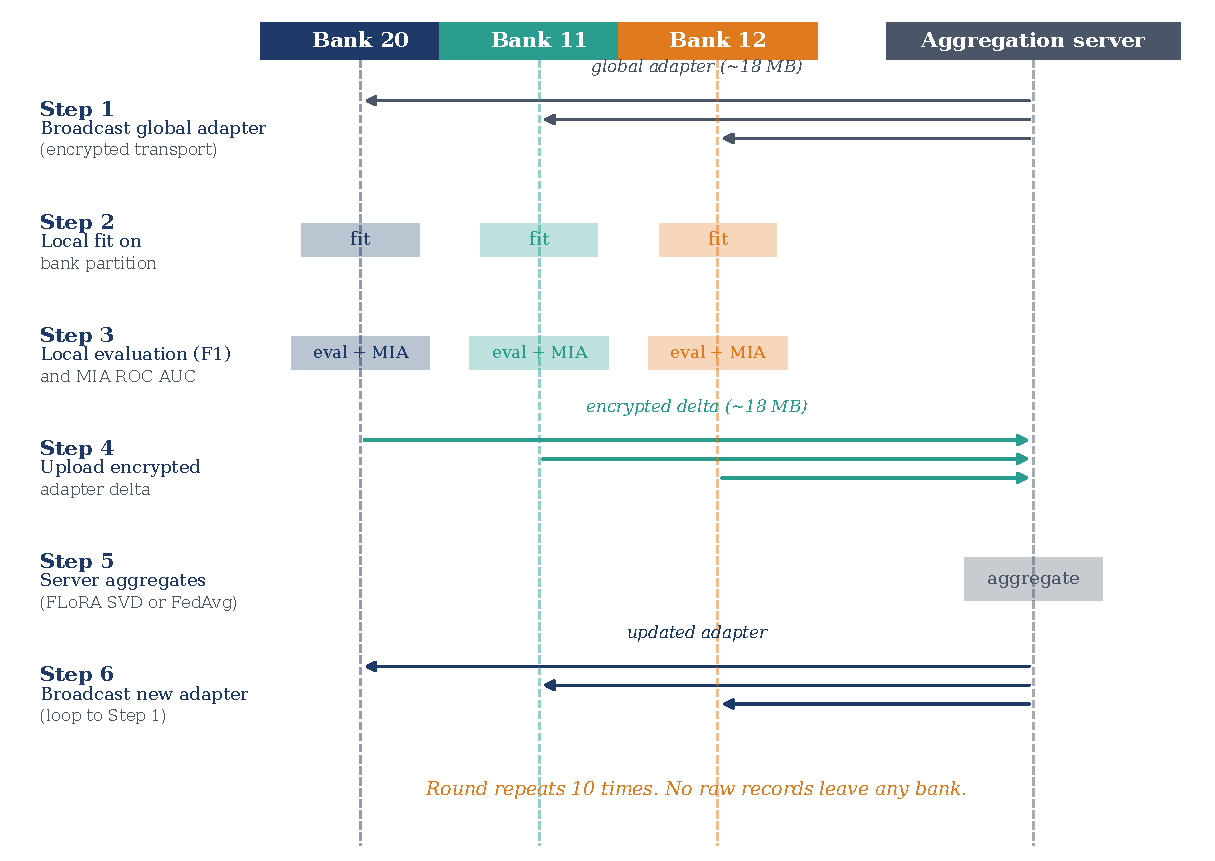
\includegraphics[width=0.95\linewidth]{res/fig-arch-federation-round.pdf}
    \caption[Sequence of messages in one federation round]{Sequence of messages in one federation round, supporting Section~\ref{sec:meth:arch} (data and control flow in one round). The three bank clients (blue, teal, orange) and the aggregation server (slate) exchange six messages per round: weight broadcast, local fit, local evaluate, membership inference attack, encrypted upload of the updated adapter, and server-side aggregation (FLoRA stacking + SVD or FedAvg parameter-wise mean). Payload sizes are annotated where informative: the adapter upload is approximately 18~MB per client per round, nearly three orders of magnitude smaller than the 16~GB per client per round (fp16) that full-weight FedAvg on the 8B backbone would transmit.}
    \label{fig:arch-federation-round}
\end{figure}

\section{Implementation}
\label{sec:meth:impl}

\subsection{Model stack}

The backbone is DeepSeek-R1-Distill-Llama-8B, loaded with \texttt{transformers} under 4-bit NF4 quantisation via \texttt{bitsandbytes} and the QLoRA recipe of Dettmers et al.~\cite{dettmers2024qlora}. A LoRA adapter~\cite{hu2021lora} is attached using the PEFT library, with rank $r=8$, scaling factor $\alpha=16$, dropout 0.05, and target modules \texttt{q\_proj} and \texttt{v\_proj}. This configuration matches the defaults used in the published FLoRA paper~\cite{flora2024federated} and is the configuration validated by the 2026-04 benchmark archived under the \texttt{benchmark-2026-04-02} tag. Extending the target set to include the full attention block and the feed-forward projections (\texttt{k\_proj, o\_proj, gate\_proj, up\_proj}) and raising the rank to $r=16$ is a natural follow-up that is supported by the current code defaults but was not re-benchmarked within the project timeline; Chapter~\ref{ch:conclusions} identifies it as a future-work item.

The base model is frozen throughout training; only the adapter parameters receive gradients. The trainable count is approximately $3.4$~million parameters, which in fp32 is $13.6$~MB of raw adapter weights and inflates to roughly $18$~MB per client per round after the Fernet authenticated-encryption wrapper (HMAC plus base64 framing). The corresponding classical FedAvg reference for the 8-billion-parameter backbone is approximately $16$~GB per client per round at fp16, nearly three orders of magnitude larger. The reduction claimed in Section~\ref{sec:bg:peft} is thus a direct consequence of the adapter configuration.

\subsection{Data ingestion and partitioning}

\texttt{src/data/aml\_ingestor.py} reads the IBM AML CSV~\cite{weber2018scalablegraphlearningantimoney} and emits account-level records annotated with the ground-truth laundering label. Partitioning by \texttt{From Bank} yields three natural cross-silo partitions, corresponding to banks with identifiers 20, 11, and 12 in the small-scale release of the dataset; these are the top three banks in the dataset by suspicious-account count (66, 64, and 36 respectively, against 26 for the fourth-ranked bank) and therefore the only partitions large enough to support the 50-member / 50-non-member MIA sampling and the balanced training mini-batches described below. For each partition the ingestor computes a stratified 70/15/15 train/validation/test split, preserving the (highly imbalanced) laundering rate of approximately 1-2 per cent in every split. The training, validation, and test partitions are materialised as disjoint Kuzu databases under \texttt{data/kuzu\_dbs/}, so that retrieval queries at evaluation time cannot leak training transactions into the test prompt.

\subsection{Graph backends}

The \texttt{KuzuGraphStore} backend stores nodes for accounts and edges for transactions, each annotated with timestamp, amount, currency, and payment type. Ingestion is executed in a single transaction per partition for speed. Retrieval is performed by Cypher-style queries over a one- or two-hop neighbourhood of the target account.

The \texttt{NetworkXGraphStore} backend implements the same interface against an in-memory \texttt{DiGraph}. It is used in the unit-test suite (Section~\ref{sec:meth:testing}) to verify that pattern detection produces identical outputs on hand-constructed graphs, and to provide a quick sanity-check path that does not depend on the Kuzu binary.

The \texttt{Neo4jGraphStore} backend speaks Cypher against a local Neo4j server. It is exercised only in smoke tests; the benchmark uses Kuzu throughout.

\subsection{Bank-scoped pattern detection}
\label{sec:meth:impl:patterns}

The module \texttt{src/graph/patterns.py} translates structural graph queries into named, LLM-digestible AML typologies. Five patterns are detected:

\begin{itemize}
    \setlength\itemsep{0em}
    \item \textbf{Pass-through}: an incoming payment of amount $X$ matched by an outgoing payment of amount in $[0.9X, 1.1X]$ within 48~hours.
    \item \textbf{Structuring}: three or more outgoing transactions to the same destination with relative standard deviation below 0.2 and individual amount below 10{,}000 USD, the threshold at which many reporting regimes require additional documentation.
    \item \textbf{Fan-out}: an account that sends to five or more distinct destinations within a short window.
    \item \textbf{Rapid-burst}: three or more outgoing transactions within one hour.
    \item \textbf{Intra-bank cycle}: a two-hop chain whose terminal node is a known sender back to the origin within the same partition.
\end{itemize}

Each pattern's detection is confined to the target account's own partition. The retrieval query never crosses into another bank's graph shard. This is the architectural guarantee that gives the RAG layer its privacy property: a node can inject rich structural context into its own prompts without ever observing transactions from another node. In the terminology of the poster, the \textit{Brain} learns globally while the \textit{Memory} stays strictly local.

Detected patterns are formatted as short English phrases, e.g. \enquote{STRUCTURING: 3 amounts between 9{,}700 and 9{,}800, all just below the 10{,}000 reporting threshold}. These phrases are injected into the prompt under a dedicated \texttt{AML Structural Signals} header, appearing after the raw transaction list that is always present in both retrieval modes.

\subsection{Retrieval modes: flat vs RAG}

Two retrieval modes are supported via \texttt{Config.retrieval\_mode}:

\begin{itemize}
    \setlength\itemsep{0em}
    \item \texttt{flat}: the prompt contains only the raw list of the target account's transactions, formatted as one line per transaction (direction, amount, currency, counterparty, timestamp, payment method). No pattern summary is included.
    \item \texttt{rag}: the prompt contains the same raw list, followed by the structural signals produced by the pattern detector.
\end{itemize}

Both modes share the same backbone, the same system prompt (which instructs the model to emit a verdict-first response), and the same decoding configuration. They differ only in whether the \texttt{AML Structural Signals} block is present. This design, illustrated in Figure~\ref{fig:arch-prompt-construction}, isolates the contribution of retrieval-augmented context from every other variable in the pipeline, and it is the basis of the ablation analysis in Chapter~\ref{ch:results}.

\begin{figure}[t]
    \centering
    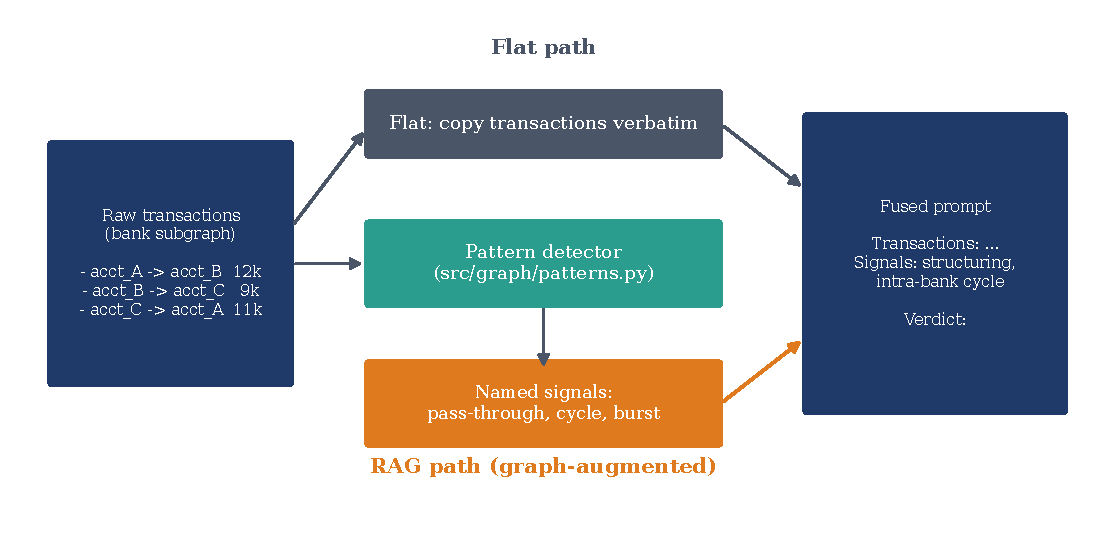
\includegraphics[width=0.95\linewidth]{res/fig-arch-prompt-construction.pdf}
    \caption[From raw transactions to a RAG prompt]{Prompt construction for the two retrieval modes, supporting Section~\ref{sec:meth:impl} (retrieval modes) and Section~\ref{sec:meth:impl:patterns} (pattern detection). Both modes begin with the same raw transaction list for the target account. In \texttt{flat} mode the prompt ends there. In \texttt{rag} mode the bank-scoped pattern detector scans the target account's local neighbourhood in the Kuzu graph store, emits named AML typologies (pass-through, structuring, fan-out, rapid-burst, intra-bank cycle), and appends them under an \texttt{AML Structural Signals} header. The pattern detector never crosses into another bank's partition.}
    \label{fig:arch-prompt-construction}
\end{figure}

\subsection{Federation client}

\texttt{src/federation/client.py} implements an in-process federated client (mirroring Flower's client interface but not using the Flower runtime, for the reasons described in Section~\ref{sec:bg:fl}) whose \texttt{fit} step is responsible for one local epoch of training, and whose \texttt{evaluate} step is responsible for both the utility metric and the membership inference AUC.

Training uses AdamW with learning rate $2 \times 10^{-4}$ and a batch size of one, the latter imposed by the GPU memory budget of a single A100 instance that also holds the 4-bit backbone, the adapter, and the Kuzu database handle. Each round samples 100 accounts from the client's training partition, forced to a 50/50 suspicious/clean ratio through oversampling with replacement of the minority class (this step is necessary because the raw class imbalance of 1-2 per cent makes unbiased sampling produce rounds with zero positives). Evaluation runs against each client's full stratified test split, which after the 70/15/15 partitioning described above yields between 380 and 726 accounts per client (averaging 578 across the three banks in the benchmark); this is the most rigorous eval setting the pipeline supports and is preferred over a sub-sampled balanced eval for the reported benchmark. Gradient accumulation was considered but not enabled in the current benchmark, and is identified as a future-work item in Chapter~\ref{ch:conclusions}.

\subsection{Training targets}
\label{sec:meth:impl:targets}

The target text for a suspicious account in flat mode is the literal string \texttt{VERDICT: SUSPICIOUS} followed by end-of-sequence. For a suspicious account in RAG mode, the target is \texttt{VERDICT: SUSPICIOUS. Structural signals: <list>}, where the list is the pattern summary detected for that account. The analogous format is used for \texttt{CLEAN}.

The key design property is that the verdict token sequence always appears before any rationale. If the prompt plus response is truncated at the model's 3072-token context limit (the value configured via \texttt{Config.max\_prompt\_tokens}), the verdict survives the truncation, whereas a rationale-first format would lose the verdict and produce spurious zero scores. This verdict-first layout was introduced during the April iteration after an earlier run showed occasional F1 score~=~0 rounds caused precisely by the prompt exceeding the context budget and the verdict being cut off.

At training time, loss is computed only on the response tokens; prompt tokens have their labels set to the ignore index $-100$. This prevents the adapter from memorising any fragment of the retrieval context.

\subsection{Aggregators}

Three aggregation strategies are implemented in \texttt{src/federation/}:

\begin{itemize}
    \setlength\itemsep{0em}
    \item \textbf{FLoRA}: adapters from the three clients are stacked and reduced by truncated SVD to the configured rank, following Wang et al.~\cite{flora2024federated}. This is the primary aggregator of interest and the only one that handles rank heterogeneity correctly.
    \item \textbf{FedAvg}: the FLoRA adapter weights are averaged element-wise across clients. This is used as a baseline only; for a like-for-like comparison against the classical FedAvg of McMahan et al.~\cite{mcmahan2017communication}, the communication cost is computed as if the full backbone parameters were being exchanged, since that is what the McMahan formulation requires.
    \item \textbf{Centralised}: a single client trains on the union of all three partitions with no federation. This is the utility upper bound, at the explicit cost of the privacy guarantee.
\end{itemize}

\subsection{Decoding}

Evaluation uses greedy decoding (\texttt{do\_sample=False}) with \texttt{max\_new\_tokens=1024}. Sampling-based decoding was used in earlier iterations but produced round-to-round F1 score variation that was larger than the effect sizes being measured across conditions. Greedy decoding makes the evaluation a deterministic function of the adapter state, which is the appropriate choice for a binary classification task whose metric is the F1 score.

\subsection{Membership inference attack}
\label{sec:meth:impl:mia}

The privacy metric is a simple, widely used membership inference proxy: for 50 training accounts (members) and 50 test accounts (non-members), the client records the per-token loss under the current model and reports the ROC AUC of a threshold-based attacker that decides \enquote{member} when the loss is below a threshold. An AUC of 0.5 indicates an attacker that cannot do better than chance; a higher AUC indicates that the model leaks more information about its training set. The metric is reported per-client, per-round, so that its trajectory over the course of training can be inspected.

This proxy is explicitly acknowledged in Chapter~\ref{ch:results} as one of many possible privacy measures. It does not constitute a proof of privacy; it constitutes an empirical signal that, across the 30 client-round combinations per aggregator in the 2026-04 benchmark, the mean AUC stayed within the $0.44{-}0.45$ band (individual client-round values ranged from $0.37$ to $0.55$), close to the chance baseline of $0.5$.

\subsection{Configuration and observability}

All experimental parameters live in a single \texttt{Config} dataclass (\texttt{src/config.py}), which is serialised to \texttt{config\_<run\_name>.json} at the start of every run. Per-round metrics (training loss, F1 score, precision, recall, MIA AUC, and the wall-clock latencies of the fit, evaluate, and aggregate stages) are appended to \texttt{history\_<run\_name>.json} after each round. A run can therefore be fully reproduced by pairing an archived config with the code state at the corresponding git tag.

\section{Path to Production Deployment}
\label{sec:meth:production}

The benchmark in Chapter~\ref{ch:results} is a single-GPU simulation. This section translates the simulation's measurements into the figures a deployment engineer would need in order to put the architecture into a real cross-silo consortium: bandwidth on a real WAN link, GPU-hour budget under typical cloud pricing, the audit artefacts the model-risk regimes of Section~\ref{sec:meth:regulatory} require, and the operational concerns (key management, rollback) that the simulation deliberately abstracts away. All numerical values reported in this section are produced by \texttt{scripts/verify/verify\_production\_deployment.py}; the dissertation cites the script's outputs.

\subsection{Bandwidth on a real WAN}

The Fernet-wrapped FLoRA adapter delta measures $18{,}197{,}432$~bytes per client per round, equivalent to $145.58$~megabits. On a $100$~Mbps inter-datacentre link this transfers in $1.46$~seconds, on a $1$~Gbps link in $0.15$~seconds, and on a $10$~Gbps link in $0.01$~seconds. The mean fit-stage wall clock for the same client per round is $770.1$~seconds (FLoRA-with-RAG, archived benchmark). The compute-to-communications ratio is therefore approximately $530\times$ at $100$~Mbps, $5{,}290\times$ at $1$~Gbps, and $52{,}900\times$ at $10$~Gbps. This is the operational consequence of the bandwidth axis collapsing by nearly three orders of magnitude (Section~\ref{sec:results:efficiency}): once the federated payload is the size of a small adapter rather than the size of the backbone, network choice ceases to be a deployment constraint; the wall-clock budget is set entirely by GPU compute.

\subsection{GPU-hour budget at on-demand cloud pricing}

A full ten-round, three-client session of FLoRA-with-RAG consumes $6.42$~A100-hours at the fit stage (the dominant stage; eval, MIA, and aggregation account for under $5$~per cent of round wall clock). At publicly listed on-demand A100 pricing the per-session cost falls between USD~$6.87$ at the specialised-cloud rate of USD~$1.07$ per A100-hour and USD~$26.25$ at the AWS p4d effective rate of USD~$4.09$ per A100-hour. At a weekly retraining cadence the consortium consumes $334$~A100-hours per year, costing between USD~$357$ and USD~$1{,}365$ at the same range. These figures are deliberately quoted per consortium and per session rather than per bank, since the federated cost is dominated by the per-client fit stage and does not scale with the size of the aggregator. They are also meaningful in absolute terms: an annual training budget of less than two thousand US dollars is small enough that compute is not the constraint on whether a consortium of mid-sized banks can run this architecture.

\subsection{Audit artefacts for SS1/23 and OSFI E-23}

Both UK and Canadian model-risk regimes (Section~\ref{sec:meth:regulatory}) require that a model's lifecycle be auditable from input to decision. The reproducibility apparatus of this project emits a triple per benchmark run that is sufficient for that purpose: a serialised \texttt{Config} dataclass capturing every experimental parameter, a \texttt{history\_*.json} appending per-round per-client metrics, and an annotated git tag pinning the exact code state. A reviewer reproducing a result therefore checks out the tag, replays the configuration, and obtains the same numbers; this is the audit trail that SS1/23~\cite{prass123} and OSFI E-23~\cite{osfie23} expect a regulated institution to be able to produce on request.

\subsection{Key management and rollback}

Two operational concerns that the simulation deliberately abstracts away and that a real deployment must address are recorded here for completeness and identified as out of scope for the dissertation's own evaluation. First, the Fernet symmetric key used by the encryption layer in \texttt{src/security/encryption.py} is a single shared secret in the simulation; a production deployment would manage one client-server key per institution, with rotation handled by an HSM-backed key-management service and re-encryption on rotation, with audit logs feeding the same observability stack as the per-round metrics. Second, the simulation has no rollback path: a regression in the global adapter would be carried into the next round. A production deployment would persist each round's global adapter as an immutable artefact, gate promotion on a held-out validation F1-score threshold, and revert to the prior adapter when promotion fails. Both extensions are routine engineering, and neither alters the architectural claims of this dissertation; they are mentioned here so that the simulation's scope is not mistaken for a deployment claim.

\section{Testing and Reproducibility}
\label{sec:meth:testing}

\subsection{Unit-level verification}

The pattern detection module is verified by constructing small transaction graphs by hand and asserting that the detector labels them according to the specifications in Section~\ref{sec:meth:impl:patterns}. The graphs are expressed through the \texttt{NetworkXGraphStore} backend, which was introduced expressly for this purpose; this also provides an executable sanity check that the \texttt{GraphStore} interface is complete, since a new backend that satisfies the abstract methods is sufficient to pass the pattern tests.

\subsection{End-to-end smoke tests}

The \texttt{scripts/} directory contains small helpers that exercise the federation loop for a single round against a miniature partition, to catch integration-level regressions between the data layer, the graph layer, and the model layer. These are not a substitute for a full benchmark run, but they reliably catch issues such as tokeniser-artefact regressions (for example, the \enquote{fast tokeniser produces Ġ/Ċ artefacts} problem that is guarded against by the \texttt{Config.use\_fast\_tokenizer=False} default).

\subsection{Benchmark reproducibility}

The formal benchmark presented in Chapter~\ref{ch:results} was executed on 2~April~2026 and is archived in the project repository under \texttt{data/2026-04-02/}. Twelve JSON files are committed (six \texttt{config\_*.json}, six \texttt{history\_*.json}), corresponding to the six-condition cross of three aggregators and two retrieval modes. The exact code state that produced those numbers is pinned by the annotated git tag \texttt{benchmark-2026-04-02}, which points at commit \texttt{01a6cce}. A reviewer reproducing the results can therefore execute \texttt{git checkout benchmark-2026-04-02} and replay the notebook against the archived configurations.

\subsection{Limitations of the testing strategy}

Two limitations should be acknowledged. First, the benchmark was run once per condition rather than across multiple seeds, so no cross-seed variance is reported; the per-round variance within a single run is the only stochastic signal available. Second, since the model's training data is not auditable at the dissertation's scale, the unit tests can verify that pattern detection is correct but cannot verify that the model's verdict is \enquote{correct} in any semantic sense beyond the supervised label. These limitations are discussed further in Section~\ref{sec:results:limits} of Chapter~\ref{ch:results}.

\section{Threat Model}
\label{sec:meth:threat}

The privacy claims made elsewhere in this chapter are claims against a specific class of adversary, not absolute claims. This section enumerates the adversaries the architecture is designed to resist, the capability assumed of each, the architectural defence, and the residual risk that survives the defence. The five adversaries below are the ones that a cross-silo deployment in the AML setting would expect to face; nothing in the architecture is designed against an active byzantine adversary, and that exclusion is stated as such.

\subsection{Honest-but-curious aggregator}

\textit{Capability.} The aggregation server follows the protocol exactly but inspects every received adapter delta and every aggregated global adapter. This is the standard threat model for cross-silo federated learning and is the one the privacy boundary is principally designed against.

\textit{Defence.} Adapter deltas are Fernet-encrypted in transit (Section~\ref{sec:meth:impl}). The plaintext content of a delta is, by construction, the gradient signal of an arbitrary low-rank transformation of the local supervisory loss; it does not encode raw transactions. The membership-inference experiments in Section~\ref{sec:results:privacy} show that a threshold-based attacker observing the resulting model cannot meaningfully distinguish training accounts from test accounts.

\textit{Residual risk.} A determined honest-but-curious server with access to a stronger attacker (shadow-model construction, gradient inversion against low-rank deltas) could in principle recover more information than the threshold-based proxy does. This residual is acknowledged in Section~\ref{sec:results:limits} and is a future-work item.

\subsection{Malicious client}

\textit{Capability.} A client institution submits a deliberately crafted adapter delta intended to corrupt the global model or to extract information from it.

\textit{Defence.} The architecture relies on the FLoRA stacking-plus-SVD aggregator's smoothing effect when ranks differ across clients, but does not implement Byzantine-robust aggregation (Krum, median, or trimmed mean). In a cross-silo setting with three known and contractually bound participants this is a deliberate trade-off: the cost of a malicious client is contractual rather than algorithmic, and the operational assumption is that a participating bank does not collude against the consortium.

\textit{Residual risk.} A simple majority of malicious clients (two of three in this benchmark) would arbitrarily steer the aggregated update. The architecture does not defend against this. A genuinely cross-organisation deployment with weaker trust assumptions would substitute a Byzantine-robust aggregator and is identified as a future-work item in Chapter~\ref{ch:conclusions}.

\subsection{Insider analyst at a participating bank}

\textit{Capability.} An employee of a participating bank with legitimate access to that bank's local node attempts to extract another participating bank's records or supervisory signal.

\textit{Defence.} Each bank's graph store, pattern detector, and local adapter exist only inside that bank's privacy boundary. Other participants' raw records and structural signals are not present at any point in the local node's filesystem or process memory. The only artefact the insider can read locally is the global adapter, which is the same arbitrary low-rank transformation discussed under the honest-but-curious aggregator above.

\textit{Residual risk.} The insider could, in principle, run the same membership-inference family of attacks against the global adapter to determine which other banks' accounts trained it. The benchmark's MIA AUC at $0.44$-$0.45$ is the empirical evidence that this attack is weak in practice; it is not a proof.

\subsection{Network observer}

\textit{Capability.} A passive observer of the inter-datacentre link between any client and the aggregator captures every packet exchanged.

\textit{Defence.} The Fernet authenticated-encryption wrapper provides confidentiality and integrity over the encrypted adapter delta, so the observer sees only ciphertext. No metadata beyond round number and message size is exposed. Message size itself is round-invariant (the adapter has the same number of parameters every round), so it carries no signal about the underlying data.

\textit{Residual risk.} The observer learns the timing of communication rounds, which could be informative in tightly synchronised deployments. The architecture does not defend against traffic-analysis attacks, and a defence would require padding or fixed-cadence transmission which is out of scope for this project.

\subsection{Model-stealing party}

\textit{Capability.} A downstream consumer of the trained adapter (say, a counterparty bank that later receives the global adapter for inference use) attempts to reconstruct the participating banks' training data from the adapter weights alone.

\textit{Defence.} The adapter weights are the cumulative low-rank transformation produced by ten rounds of stacking-plus-SVD aggregation across three clients. They are not addressable by individual training examples, and the per-token loss profile they produce against a held-out account does not reliably distinguish member from non-member at the threshold-based attacker's resolution.

\textit{Residual risk.} A motivated attacker with a substantial compute budget and access to the training procedure's metadata could mount stronger reconstruction attacks. As above, the dissertation does not claim formal privacy in the differential-privacy sense; it claims that, against the threshold-based attacker that is the project's empirical privacy probe, the leakage is at chance.

\section{Ethical Considerations}
\label{sec:meth:ethics}

\subsection{Data provenance and privacy}

The IBM AML dataset is synthetic and openly licensed~\cite{weber2018scalablegraphlearningantimoney}. No real customer data was accessed during the project, and no ethics committee approval was required. The project nevertheless treats privacy as a first-class design concern because the architecture is intended to be reusable beyond the dissertation in domains where the data is not synthetic. The privacy boundary established by the local-RAG design is an architectural guarantee, not a policy declaration: raw records cannot leave a node because there is no code path that would permit them to.

\subsection{Regulatory alignment}

The architecture's relationship to the regulatory regimes governing the AML case study (GDPR Articles 5(1)(c) and 25, FATF Recommendations 10, 11 and 20, UK MLR 2017, USA PATRIOT Act \S~314(b), PRA SS1/23, OSFI Guideline E-23, and 6AMLD) is set out in Section~\ref{sec:meth:regulatory}, where each regulation is tied to the specific design decision that satisfies it. The summary point relevant to the ethics chapter is that no node transmits raw customer records: each node transmits only adapter deltas, which are (i) several orders of magnitude smaller than the underlying data, (ii) an arbitrary learned transformation of that data rather than a reversible encoding, and (iii) cryptographically protected in transit by the symmetric encryption layer in \texttt{src/security/encryption.py}.

\subsection{Model bias}

DeepSeek-R1-Distill-Llama-8B was trained on a broad web corpus whose composition is not disclosed in full. Any biases in that corpus may propagate to the model's verdicts, and the project makes no claim that the distilled model is neutral with respect to, for example, the national origin of counterparty names or the linguistic register of transaction descriptions. The F1 score evaluation is performed against supervised laundering labels that are themselves synthetic and are not audited for bias. The project does not make deployment claims; it evaluates an architectural pattern on a benchmark whose conclusions would need to be revisited before any real-world application.

\subsection{Responsible use of membership inference}

The membership inference attack implemented in Section~\ref{sec:meth:impl:mia} is configured to measure the project's \emph{own} model, using the project's own training and test sets. No externally hosted model is attacked. The MIA code is documented in the repository as a defensive measurement tool, not as a generalised attack framework, and is kept inside the same Python package so that it cannot be used against other systems without deliberate modification.

\subsection{Environmental footprint}

A single benchmark run at the scale used in this project consumes approximately nine hours of A100 GPU time across the six conditions. This is a non-trivial environmental cost that is justified here by the research contribution, but would need to be amortised across many deployments before the architecture paid for itself relative to simpler baselines. A full energy-overhead accounting in FLOPs was flagged during supervision as a useful future extension and is identified as a future-work item in Chapter~\ref{ch:conclusions}.

\subsection{Right to explanation and automated decision-making (GDPR Article~22)}

GDPR Article~22 entitles a data subject not to be subject to a decision based solely on automated processing that produces legal or similarly significant effects, with limited exceptions. An AML verdict triggering an STR is exactly such a decision: it can lead to a frozen account, a regulatory filing, or a criminal investigation. The architecture takes the same position as supervised AML monitoring systems already in deployment: the model is a triage stage, not the decision. The verdict produced by the LLM is intended as input to a human investigator, not a substitute. The verdict-first target format (Section~\ref{sec:meth:impl:targets}) is also helpful here because it makes the model's output a label rather than a free-form rationale, which keeps the audit trail short and easy to summarise to a data subject under Article~15 (right of access).

\subsection{Dual-use risk}

The bank-scoped pattern detector encodes structural typologies that are also useful to an adversary planning a laundering campaign: knowing what the detector looks for could in principle inform how to evade it. The dissertation reports the typologies because they are already documented in the FATF Recommendations~\cite{fatf2025recommendations} and in the public AML compliance literature, so the publication risk is incremental rather than novel. The detector implementation is parameterised (thresholds, time windows) so that a real deployment would tune its parameters away from the published defaults; this is the standard mitigation in the AML monitoring space.

\subsection{Fairness considerations under deployment}

The dissertation does not run a fairness audit against protected characteristics (national origin, age, gender) because the IBM AML dataset is synthetic and does not carry the relevant attributes. A real deployment would need to run such an audit before promotion, and the audit artefacts already produced (per-client per-round JSON, pinned git tag) are the right substrate for it: the same per-account predictions can be re-grouped by any protected attribute the deployment's own data carries, and the model can be retrained or recalibrated if disparate impact appears. The architecture does not preclude a fairness layer; it does not implement one either, and that omission is stated explicitly here.

\subsection{Use of generative AI in the authoring process}

Generative AI tooling (commercial LLM assistants) was used during the preparation of this dissertation to improve spelling, phrasing, grammar, and academic writing style, and to suggest figure layouts and table structures. All technical claims, numerical values, and regulatory citations were verified by the author against primary sources or against the verification scripts under \texttt{scripts/verify/}; the AI tooling did not generate experimental results, did not compute reported numbers, and did not produce the bibliography. The benchmark itself was executed by the author on a Colab A100 instance and is reproducible from the pinned git tag \texttt{benchmark-2026-04-02}.

\section{Deviations from the Project Proposal}
\label{sec:meth:deviations}

The following deviations from the March project proposal occurred during implementation. Each is reported with its cause and its effect on the research contribution, in keeping with the rubric's expectation that the methodology chapter account honestly for changes of plan.

\paragraph{Compute platform and federation substrate: T4 + Flower to A100 + in-process loop.} The proposal anticipated a Google Colab T4 accelerator at 16~GB VRAM and Flower's Virtual Client Engine as the simulation substrate. Flower's engine, however, schedules each client on a separate Ray worker process, and each worker pickles its own copy of the 8-billion-parameter backbone alongside the activations, gradient-checkpointing buffers, AdamW optimiser state, and KV cache that one fine-tuning round requires. Although the quantised backbone fits in approximately 6~GB at 4-bit NF4, three concurrent workers compound this footprint past the 40~GB A100 budget and trigger OOM. The project therefore made two deviations in tandem: (i) the simulation was re-implemented as a bespoke in-process loop that loads the base model once and shares it by reference across clients, keeping Flower's client interface as the design template; and (ii) the compute platform was migrated to a Colab A100 instance at 40~GB VRAM for simulation headroom. The architectural claim is unaffected: production deployments in which each bank has its own dedicated accelerator would not face the same simulation-specific constraint.

\paragraph{Retrieval terminology, \enquote{graph} to \enquote{RAG}.} The proposal described the experimental axis as \enquote{flat versus graph}. During implementation it became clear that the relevant distinction is between flat prompts and retrieval-augmented prompts, not between flat prompts and a raw graph dump. The axis was therefore renamed to \enquote{flat versus RAG} in the dissertation's prose and in future configurations. The archived 2026-04 benchmark configurations retain the earlier \texttt{retrieval\_mode: "graph"} label for compatibility with the exported JSON files; the semantics are identical. The module path \texttt{src/graph/} and the \texttt{GraphStore} interface were deliberately not renamed, because they refer to the database abstraction, not to the retrieval axis.

\paragraph{Evaluation sample size.} The proposal did not commit to an evaluation sample size. Early smoke runs used a single account per client per round, which was sufficient for integration testing but would have produced too much round-to-round F1 score variance to support cross-condition claims. The benchmark presented in Chapter~\ref{ch:results} instead evaluates each client against its full stratified test split (between 380 and 726 accounts per client depending on the bank, averaging 578 across the three banks), which is the most rigorous option supported by the pipeline and which yields F1-score estimates whose round-to-round variance is well below the effect sizes separating the six conditions.

\paragraph{Training target format and decoding.} The proposal did not commit to either a target format or a decoding strategy. Early runs used a rationale-first target and sampling-based decoding; both were identified during the April iteration as sources of instability. The benchmark reported here uses a verdict-first target (so that prompt truncation cannot remove the verdict) and greedy decoding (so that evaluation is deterministic). Both changes are documented in Sections~\ref{sec:meth:impl:targets} and in the implementation prose above.

\chapter{Results and Evaluation}
\label{ch:results}

\section*{How to read this chapter}

The chapter reports the six-condition benchmark introduced in Chapter~\ref{ch:method}: three aggregators (centralised, FedAvg, FLoRA) crossed with two retrieval modes (flat, RAG), ten federation rounds per condition, three bank clients per round. The reading flow is intentionally linear so that a reader who has not seen the architecture before still leaves the chapter able to answer the four questions that drive the rest of the dissertation.

\textit{What was measured?} Section~\ref{sec:results:setup} states the experimental setup and defines the three evaluation criteria (F1 score, communication volume plus per-stage wall-clock, membership-inference AUC) so that the figures and tables that follow are unambiguous.

\textit{Where do the trilemma axes land?} Sections~\ref{sec:results:utility}, \ref{sec:results:efficiency}, and~\ref{sec:results:privacy} report one axis each, in the order utility-then-efficiency-then-privacy that mirrors the dissertation's headline argument.

\textit{Does retrieval matter?} Section~\ref{sec:results:ablation} isolates the contribution of RAG by pairing each aggregator's flat and RAG runs.

\textit{What does this cost in operations?} Section~\ref{sec:results:cost} translates the F1 score into projected investigator workload and dollar cost per million transactions, reading the trilemma in the units that matter to a deployment.

The chapter closes in Section~\ref{sec:results:limits} with a self-audit of the limitations of the evaluation, which the conclusions chapter then picks up as future-work items. The order of presentation is deliberate: a reader who screens only the section headings still sees the chapter argue that the FLoRA-with-RAG configuration meets every acceptance condition stated in Section~\ref{sec:results:eval-criteria}, that the retrieval mode contributes a measurable lift in peak F1 score, and that the operational cost of the configuration is dominated by alert investigation rather than by training compute.

Every figure is produced from the archived JSON files under \texttt{data/2026-04-02/} by the scripts under \texttt{scripts/figures/}, and is reproducible from the pinned commit \texttt{01a6cce} (git tag \texttt{benchmark-2026-04-02}, repository \url{https://github.com/SlaviXG/thinking-inside-the-box}). Numerical claims in the prose, including the cost projections of Section~\ref{sec:results:cost} and the production-deployment figures cross-referenced from Chapter~\ref{ch:method}, are re-derived independently by the scripts under \texttt{scripts/verify/}.

\section{Experimental Setup}
\label{sec:results:setup}

\subsection{Configuration shared across all six runs}

All six runs share the same backbone (DeepSeek-R1-Distill-Llama-8B at 4-bit NF4), the same LoRA configuration ($r=8$, $\alpha=16$, targets \texttt{q\_proj}+\texttt{v\_proj}), the same optimiser (AdamW, learning rate $2 \times 10^{-4}$, batch size one), and the same per-round budget (100 balanced training samples, full stratified test split evaluation, 50 members and 50 non-members for MIA), as summarised in Table~\ref{tab:config-summary}. They differ only in the aggregation strategy and the retrieval mode. Every run is ten rounds long and distributes three clients across the IBM AML partitions for banks 20, 11, and 12.

% Auto-generated by scripts/figures/make_tables.py; do not edit by hand.
\begin{table}[t]
\centering
\caption[Benchmark hyper-parameter summary]{Benchmark hyper-parameters used for the 2026-04-02 run. Values are taken from \texttt{data/2026-04-02/config\_flora\_graph.json}; other conditions share all values except \texttt{retrieval\_mode} and \texttt{aggregation}.}
\label{tab:config-summary}
\begin{tabular}{ll}
\toprule
Parameter & Value \\
\midrule
Backbone & \texttt{deepseek-ai/DeepSeek-R1-Distill-Llama-8B} \\
Quantisation & 4-bit \\
LoRA rank & 8 \\
LoRA alpha & 16 \\
LoRA dropout & 0.05 \\
Federation rounds & 10 \\
Clients & 3 \\
Local epochs & 1 \\
Learning rate & 0.0002 \\
Train samples per client & 100 \\
Eval set per client & full stratified test split (380--726, mean 578) \\
MIA members & 50 \\
MIA non-members & 50 \\
Retrieval limit & 20 \\
Retrieval depth & 2 \\
Graph backend & kuzu \\
\bottomrule
\end{tabular}
\end{table}


\subsection{Evaluation criteria}
\label{sec:results:eval-criteria}

Three evaluation criteria are reported, one per axis of the trilemma. All three are computed per round per client and aggregated across clients for the figures in this chapter; the per-client values are also retained in the archived JSON for downstream inspection.

\textit{Utility: F1 score.} The F1 score~\cite{10.3115/1072064.1072067} is the harmonic mean of precision $P = \mathrm{TP}/(\mathrm{TP}+\mathrm{FP})$ and recall $R = \mathrm{TP}/(\mathrm{TP}+\mathrm{FN})$ on the binary suspicious-account label, computed as $\mathrm{F1} = 2PR/(P+R)$. The choice of F1 score over plain accuracy is motivated by the dataset's class imbalance: the IBM AML positive-class rate is $1.5\%$, so a constant ``clean'' classifier would achieve $98.5\%$ accuracy and $0$ F1 score. F1 score weights false positives and false negatives equally; the cost analysis in Section~\ref{sec:results:cost} re-weights these for the operational case.

\textit{Efficiency: communication volume and per-stage wall-clock.} Communication volume is reported as bytes transferred per client per round. The FLoRA payload is the size of the Fernet-wrapped adapter delta as written to the wire by \texttt{src/security/encryption.py}; the FedAvg reference is the McMahan formulation, which broadcasts the full backbone parameters at fp16. Wall-clock latency is reported per round, decomposed into the fit, evaluate, MIA, and aggregation stages. Each stage is timed inside the federated client loop using \texttt{time.perf\_counter} and persisted to the per-round JSON.

\textit{Privacy: membership-inference AUC.} The privacy probe is a threshold-based membership-inference attacker. For each client and each round, the client computes the per-token language-modelling loss against $50$ training-set accounts (members) and $50$ test-set accounts (non-members). The Receiver Operating Characteristic Area Under the Curve (ROC AUC) of an attacker that classifies an account as ``member'' when its loss is below a threshold is reported as the privacy metric. An AUC of $0.5$ corresponds to an attacker that cannot do better than chance; values above $0.5$ indicate leakage. The proxy is conservative by construction (a stronger shadow-model attacker may recover more); the limitation is acknowledged in Section~\ref{sec:results:limits}.

\textit{Acceptance condition.} For each axis the dissertation states the acceptance condition that an architecture must meet to be operationally interesting in this setting. Utility: F1 score within $0.10$ of the centralised-flat upper bound. Efficiency: per-client per-round payload at least two orders of magnitude below the McMahan fp16 reference. Privacy: membership-inference AUC within $\pm 0.10$ of the chance baseline. The reported FLoRA-with-RAG configuration satisfies all three.

\section{Utility: F1 Score Across Conditions}
\label{sec:results:utility}

% Auto-generated by scripts/figures/make_tables.py; do not edit by hand.
\begin{table}[t]
\centering
\caption[Per-round F1 across all six conditions]{Per-round mean F1 across the three clients for every condition in the 2026-04-02 benchmark. The per-column peak round is emphasised in bold. Columns are grouped by aggregator (Centralised, FedAvg, FLoRA) with the two retrieval modes (flat, RAG) reported side by side.}
\label{tab:f1-per-round}
\small
\begin{tabular}{c rr rr rr}
\toprule
 & \multicolumn{2}{c}{Centralised} & \multicolumn{2}{c}{FedAvg} & \multicolumn{2}{c}{FLoRA} \\
\cmidrule(lr){2-3} \cmidrule(lr){4-5} \cmidrule(lr){6-7}
Round & flat & RAG & flat & RAG & flat & RAG \\
\midrule
R1 & 0.409 & 0.000 & 0.640 & 0.317 & 0.681 & 0.444 \\
R2 & 0.667 & 0.774 & 0.637 & 0.477 & 0.627 & 0.413 \\
R3 & 0.528 & 0.564 & 0.725 & 0.333 & 0.515 & 0.455 \\
R4 & 0.676 & 0.704 & 0.672 & 0.500 & 0.701 & 0.343 \\
R5 & 0.692 & 0.077 & 0.722 & 0.638 & 0.702 & 0.753 \\
R6 & 0.526 & 0.787 & 0.667 & 0.758 & \textbf{0.740} & \textbf{0.805} \\
R7 & 0.821 & \textbf{0.844} & 0.657 & 0.759 & 0.700 & 0.717 \\
R8 & 0.756 & 0.836 & \textbf{0.756} & 0.742 & 0.724 & 0.593 \\
R9 & 0.727 & 0.650 & 0.712 & 0.744 & 0.663 & 0.676 \\
R10 & \textbf{0.852} & 0.632 & 0.643 & \textbf{0.781} & 0.680 & 0.630 \\
\bottomrule
\end{tabular}
\end{table}


Figure~\ref{fig:f1-rounds} shows the per-round mean F1-score trajectories across the three clients, and Table~\ref{tab:f1-per-round} reports the exact per-round values that underlie the figure for direct numerical inspection. The centralised-flat baseline establishes the utility upper bound at F1 score~$=0.852$ and stabilises from round three onwards; the primary configuration of interest, FLoRA with RAG, peaks at F1 score~$=0.805$ (within $0.05$ of that bound) before settling at F1 score~$=0.630$ on the final round, while FedAvg with RAG converges more cleanly to F1 score~$=0.781$. The training-loss curves in Figure~\ref{fig:train-loss} are still descending by round ten (falling from approximately $0.22$ to $0.08$ across aggregators), indicating that the six federated conditions are budget-limited rather than plateaued; the peak-versus-final split in Figure~\ref{fig:peak-vs-final-f1} and Table~\ref{tab:peak-final-f1} captures this distinction explicitly, including the round at which each condition achieved its peak. The per-client trajectory in Figure~\ref{fig:per-client-f1} shows that cross-silo heterogeneity dominates: individual-client F1 score under FLoRA with RAG averages between $0.52$ and $0.64$ despite per-client peaks of $0.78$ to $0.83$, consistent with the three banks' differing test-split sizes (380, 629, 726 accounts). Figure~\ref{fig:precision-recall-f1} disentangles whether a condition reaches its F1 through high precision or high recall: centralised-flat and FedAvg-with-RAG both finish with recall at or above $0.90$, whereas FLoRA-with-RAG finishes in a balanced $P \approx R \approx 0.63$ regime, which is the more conservative operational profile for an AML deployment.

\begin{figure}[t]
    \centering
    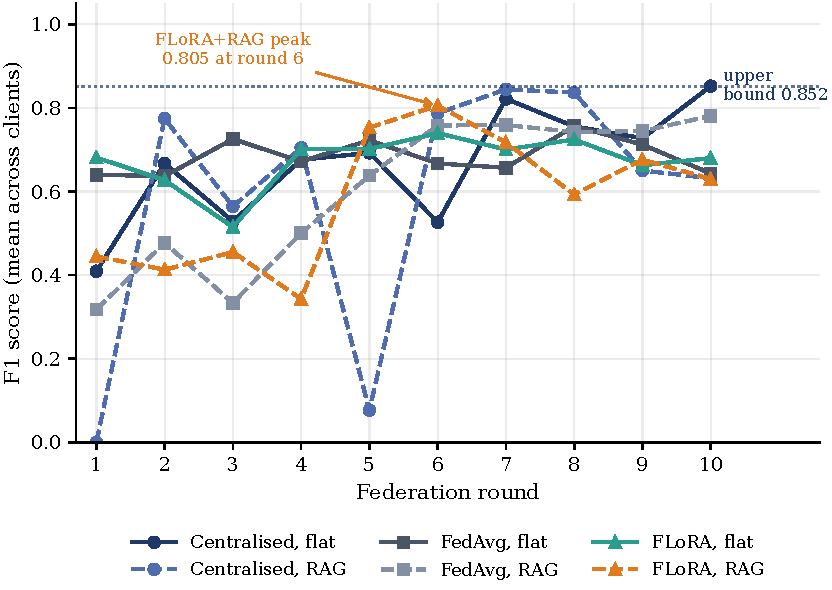
\includegraphics[width=0.92\linewidth]{res/fig-f1-rounds.pdf}
    \caption[Per-round F1 score across six conditions]{Per-round mean F1 score across the three clients for every condition. Solid lines denote \texttt{flat} retrieval; dashed lines denote \texttt{rag}. The centralised-flat baseline sets the utility upper bound; FLoRA-with-RAG is the primary configuration of interest.}
    \label{fig:f1-rounds}
\end{figure}

\begin{figure}[t]
    \centering
    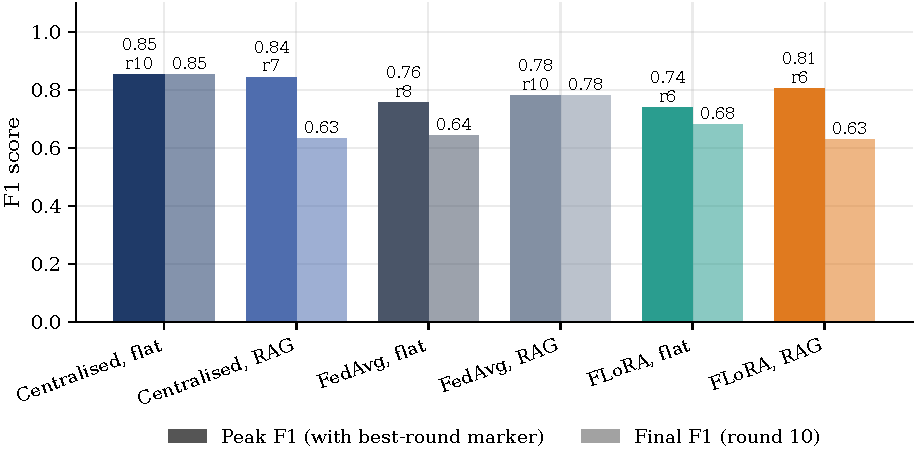
\includegraphics[width=0.92\linewidth]{res/fig-peak-vs-final-f1.pdf}
    \caption[Peak and final-round F1 score per condition]{Peak and final-round F1 score per condition, averaged across clients. The peak F1 score captures the best the configuration reaches within the ten-round budget; the final F1 score captures where the run stabilises. The pair is reported because training over a single budget can plateau short of its peak.}
    \label{fig:peak-vs-final-f1}
\end{figure}

% Auto-generated by scripts/figures/make_tables.py; do not edit by hand.
\begin{table}[t]
\centering
\caption[Peak and final F1 per condition]{Peak F1, round of peak, and final-round F1 for each condition in the 2026-04-02 benchmark (\texttt{data/2026-04-02}).}
\label{tab:peak-final-f1}
\begin{tabular}{lccc}
\toprule
Condition & Peak F1 & Round of peak & Final F1 \\
\midrule
Centralised, flat & 0.852 & 10 & 0.852 \\
Centralised, RAG & 0.844 & 7 & 0.632 \\
FedAvg, flat & 0.756 & 8 & 0.643 \\
FedAvg, RAG & 0.781 & 10 & 0.781 \\
FLoRA, flat & 0.740 & 6 & 0.680 \\
FLoRA, RAG & 0.805 & 6 & 0.630 \\
\bottomrule
\end{tabular}
\end{table}


\begin{figure}[t]
    \centering
    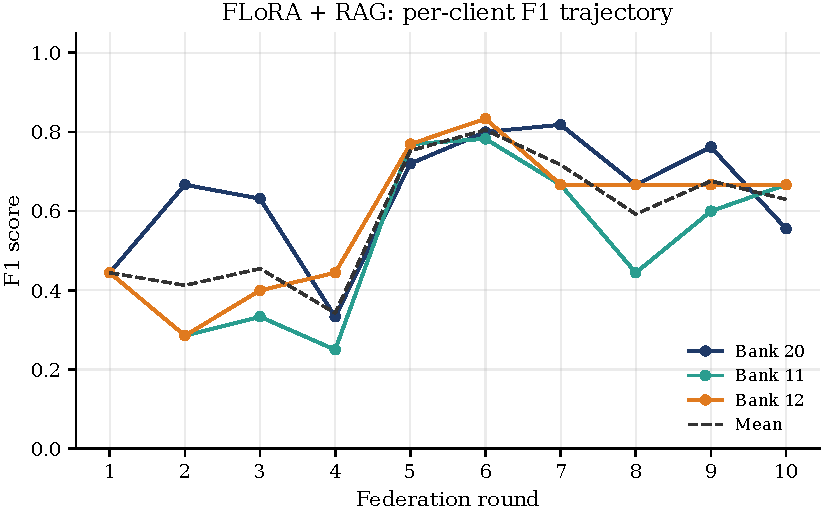
\includegraphics[width=0.92\linewidth]{res/fig-per-client-f1.pdf}
    \caption[Per-client F1-score trajectory for FLoRA with RAG]{Per-client F1-score trajectory under FLoRA with RAG. Each line is one of the three banks; the dashed grey line is the cross-client mean. Per-client curves are reported because cross-silo heterogeneity, not cross-round variance, is the main source of spread in the benchmark.}
    \label{fig:per-client-f1}
\end{figure}

\begin{figure}[t]
    \centering
    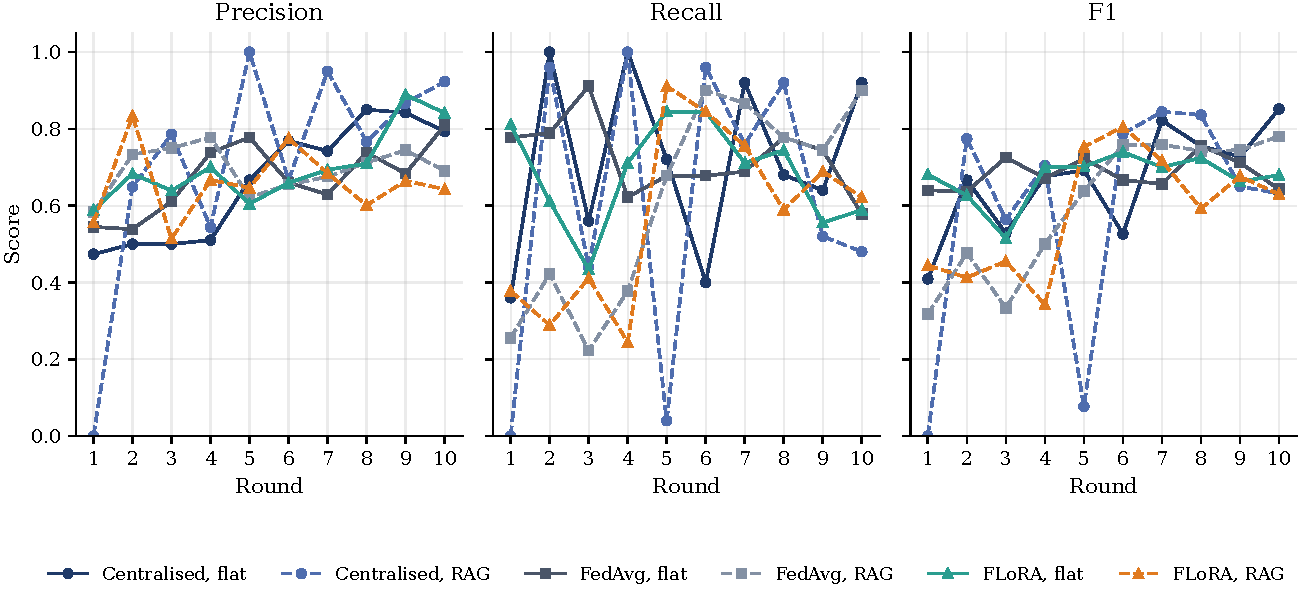
\includegraphics[width=0.92\linewidth]{res/fig-precision-recall-f1.pdf}
    \caption[Precision, recall, and F1 score across conditions]{Precision, recall, and F1 score reported separately. Plotting the three together clarifies whether a condition reaches a high F1 score by being conservative (high precision, low recall) or aggressive (high recall, lower precision); the two failure modes carry different operational consequences in an AML deployment.}
    \label{fig:precision-recall-f1}
\end{figure}

\begin{figure}[t]
    \centering
    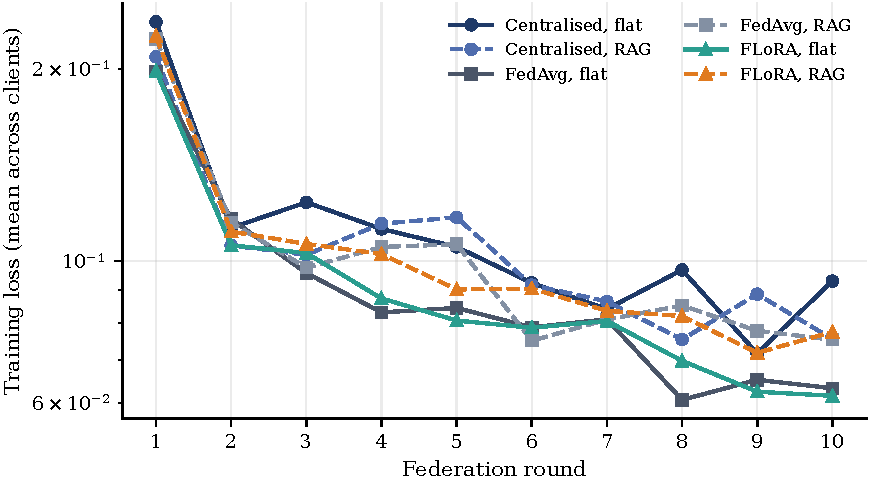
\includegraphics[width=0.92\linewidth]{res/fig-train-loss.pdf}
    \caption[Training loss per round]{Mean per-round training loss across clients for every condition. The loss curves are the clearest evidence that the adapters are learning; F1-score dynamics in the preceding figures are a downstream consequence.}
    \label{fig:train-loss}
\end{figure}

\section{Efficiency: Communication Volume and Wall-clock Latency}
\label{sec:results:efficiency}

Figure~\ref{fig:comms-volume} reports the raw bandwidth advantage: a FLoRA round transmits approximately $18$~MB of Fernet-encrypted adapter deltas per client, against the approximately $16$~GB a McMahan-style FedAvg round would transmit if the full 8B backbone were broadcast at fp16, a reduction close to $880\times$. The FLoRA figure is a measured value taken from the archive; the FedAvg figure is the theoretical McMahan reference, since the simulation aggregates weights in-process rather than over a physical link. Wall-clock time, however, tells a different story. Figure~\ref{fig:latency-stack} decomposes each round into fit, evaluate, MIA, and aggregation stages, and shows that the fit stage dominates every federated condition: approximately $770$--$800$~s per round for FLoRA, $140$--$165$~s for FedAvg, and $55$--$62$~s for the centralised baseline. The consequence is that the efficiency saving realised here is a bandwidth saving, not a time saving; once a single client runs a LoRA-fine-tuning epoch against the 8B backbone, per-round latency is set by GPU compute rather than by the network payload. This is consistent with the trilemma-decoupling thesis: the architecture separates communication cost from compute cost, and the two axes are reported independently rather than conflated.

\begin{figure}[t]
    \centering
    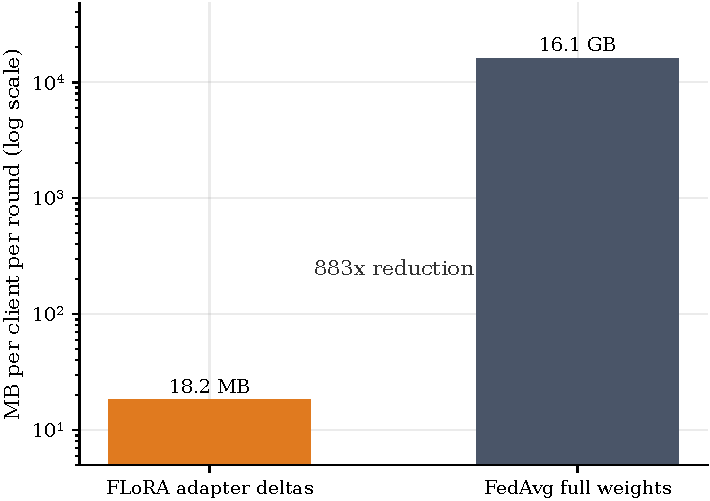
\includegraphics[width=0.88\linewidth]{res/fig-comms-volume.pdf}
    \caption[Communication volume per round]{Communication volume per client per round, on a logarithmic scale in megabytes. FedAvg's figure is computed as if the full backbone were transmitted (the McMahan formulation); FLoRA transmits only the adapter delta. The resulting reduction is approximately three orders of magnitude, consistent with the claim in Section~\ref{sec:bg:peft}.}
    \label{fig:comms-volume}
\end{figure}

\begin{figure}[t]
    \centering
    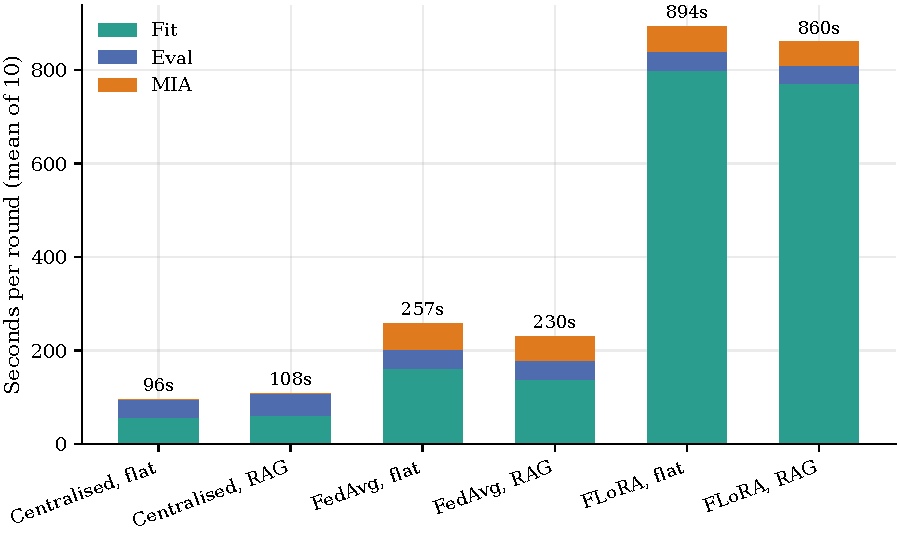
\includegraphics[width=0.88\linewidth]{res/fig-latency-stack.pdf}
    \caption[Wall-clock latency breakdown]{Wall-clock latency per round, decomposed into the fit, evaluate, membership-inference, and aggregation stages. Reporting the stages separately is the only way to show that, although communication volume collapses with FLoRA, the fit stage remains the wall-clock bottleneck because each client runs a local epoch of LoRA fine-tuning against the 8B backbone.}
    \label{fig:latency-stack}
\end{figure}

\section{Privacy: Membership Inference AUC}
\label{sec:results:privacy}

Figure~\ref{fig:mia-auc} plots the threshold-based MIA AUC per client per round for the four federated conditions. The chance baseline is $0.5$; the run-averaged mean AUCs are $0.442$ for FedAvg-flat, $0.449$ for FedAvg-with-RAG, $0.450$ for FLoRA-flat, and $0.450$ for FLoRA-with-RAG, with individual per-client per-round observations ranging from $0.367$ to $0.554$. All four means sit below chance and every observation falls within roughly $\pm 0.15$ of it, consistent with an attacker that cannot meaningfully separate members from non-members from the adapter losses alone. Neither the aggregator choice nor the retrieval mode shifts the AUC outside this near-chance band, which is the intended behaviour: the exchanged payload contains only low-rank adapter updates and is additionally Fernet-encrypted, so a threshold-based attacker has little signal to work with. The proxy attacker used here is conservative by construction, and a stronger shadow-model attack would give a more pessimistic upper bound; this limitation is stated in Section~\ref{sec:results:limits} and picked up as a future-work item in Chapter~\ref{ch:conclusions}.

\begin{figure}[t]
    \centering
    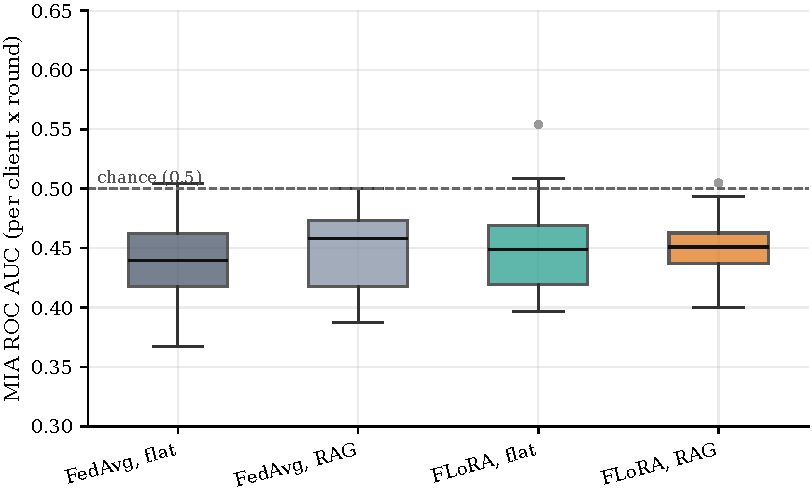
\includegraphics[width=0.92\linewidth]{res/fig-mia-auc.pdf}
    \caption[Membership inference AUC across conditions]{Membership inference attack AUC reported per client per round. The dashed horizontal line at $0.5$ is the chance baseline: an attacker at that AUC cannot distinguish members from non-members. Values below $0.5$ indicate that the attacker would be wrong more often than chance, which is a benign regime for a privacy measure.}
    \label{fig:mia-auc}
\end{figure}

\section{Flat versus RAG: Ablation}
\label{sec:results:ablation}

Figure~\ref{fig:flat-vs-rag} pairs the peak and final F1 score of each aggregator under the two retrieval modes, isolating the contribution of the RAG context with every other pipeline variable held constant; Table~\ref{tab:ablation-flat-vs-rag} reports the underlying values together with the RAG-minus-flat delta on each axis. RAG lifts the peak F1 score of both federated aggregators ($+0.024$ for FedAvg and $+0.066$ for FLoRA) but leaves the centralised baseline essentially unchanged ($-0.007$), consistent with the view that RAG compensates for the smaller per-client compute budget under federation rather than adding information the centralised baseline does not already see. Final-round F1 score is more mixed: FedAvg gains the full RAG uplift ($0.643 \to 0.781$), centralised falls from $0.852$ to $0.632$ on the final round under RAG, and FLoRA-with-RAG's final-round drop relative to its own peak is large enough that flat retrieval finishes slightly higher than graph ($0.680$ versus $0.630$) - a round-to-round instability already visible in Figure~\ref{fig:f1-rounds}. The pattern suggests RAG is a reliable peak-F1-score lifter for federated training but does not, on its own, stabilise the final-round outcome, which is the reason both peak and final are reported throughout this chapter. Table~\ref{tab:trilemma-summary} consolidates the three trilemma axes into a single per-method view, putting the chapter's headline numbers next to each other so the utility, privacy, and efficiency outcomes of each method can be compared in one read.

% Auto-generated by scripts/figures/make_tables.py; do not edit by hand.
\begin{table}[t]
\centering
\caption[Trilemma summary across methods]{Trilemma summary across the six benchmarked conditions. Utility is the per-condition peak F1 from Table~\ref{tab:f1-per-round}; Privacy is the run-averaged threshold-based MIA AUC against the chance baseline of $0.5$; Efficiency is the per-client per-round payload, with the FedAvg figure being the McMahan-style fp16 backbone reference and the FLoRA figure being the measured Fernet-encrypted adapter delta from the archive. Centralised conditions have no federation boundary and therefore no MIA or comms cost.}
\label{tab:trilemma-summary}
\small
\begin{tabular}{lccl}
\toprule
Method & Utility (peak F1) & Privacy (mean MIA AUC) & Efficiency (per-client per-round) \\
\midrule
Centralised, flat & 0.852 & N/A & N/A \\
Centralised, RAG & 0.844 & N/A & N/A \\
FedAvg, flat & 0.756 & 0.442 & 16.1~GB (1$\times$ baseline) \\
FedAvg, RAG & 0.781 & 0.449 & 16.1~GB (1$\times$ baseline) \\
FLoRA, flat & 0.740 & 0.450 & 18.2~MB (883$\times$ vs FedAvg) \\
FLoRA, RAG & 0.805 & 0.450 & 18.2~MB (883$\times$ vs FedAvg) \\
\bottomrule
\end{tabular}
\end{table}


\begin{figure}[t]
    \centering
    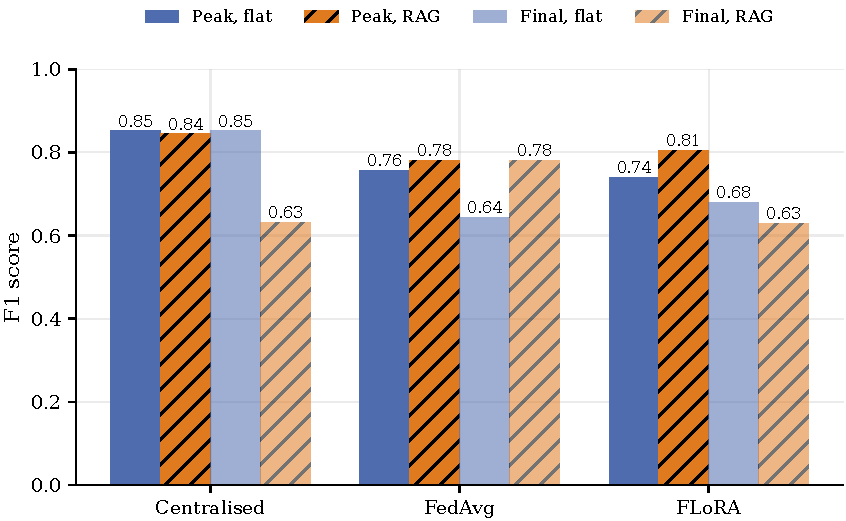
\includegraphics[width=0.88\linewidth]{res/fig-flat-vs-rag.pdf}
    \caption[Flat vs RAG, paired per aggregator]{Flat vs RAG, paired per aggregator. Each pair of bars reports peak and final F1 score for the same aggregator under the two retrieval modes. The figure isolates the contribution of the retrieval-augmented context, holding every other pipeline variable constant.}
    \label{fig:flat-vs-rag}
\end{figure}

% Auto-generated by scripts/figures/make_tables.py; do not edit by hand.
\begin{table}[t]
\centering
\caption[Flat vs RAG ablation]{Flat vs RAG ablation: peak and final F1 per aggregator, with the RAG minus flat delta. A positive delta means adding the graph-based signals helped.}
\label{tab:ablation-flat-vs-rag}
\begin{tabular}{lrrrrrr}
\toprule
Aggregator & Peak flat & Peak RAG & $\Delta$ peak & Final flat & Final RAG & $\Delta$ final \\
\midrule
Centralised & 0.852 & 0.844 & -0.007 & 0.852 & 0.632 & -0.220 \\
Fedavg & 0.756 & 0.781 & 0.024 & 0.643 & 0.781 & 0.138 \\
Flora & 0.740 & 0.805 & 0.066 & 0.680 & 0.630 & -0.050 \\
\bottomrule
\end{tabular}
\end{table}


\section{Operational Cost: Projecting the Trilemma onto Investigation Budgets}
\label{sec:results:cost}

The utility, efficiency, and privacy axes reported above are intrinsic measurements of the model. The operational consequence at deployment time is dominated by a different number: how many alerts an analyst has to investigate per period, and what fraction of those are false. AML investigations are widely reported to cost on the order of USD~30-70 per alert in the LexisNexis True Cost of Financial Crime Compliance series and aligned industry analyses, with 85-95\% of monitoring alerts ultimately resolving as false positives. This subsection projects the benchmark's measured precision and recall onto a reference monitoring volume of one million transactions, holding the dataset's empirical positive-class rate of 1.5\% fixed, so that the trilemma trade-offs can be read in investigator-budget units rather than F1-score units. The full computation is performed by \texttt{scripts/verify/verify\_cost\_of\_misclassification.py}; the dissertation reports its outputs.

The projection model is the simplest one consistent with a binary classifier whose precision and recall are known: at a positive-class rate $p_{\text{true}}$, monitored volume $V$, recall $R$, and precision $P$, the implied counts per period are $\text{TP} = V p_{\text{true}} R$, $\text{FP} = \text{TP}(1 - P)/P$, and $\text{FN} = V p_{\text{true}}(1 - R)$. The investigation cost upper bound is then $\text{FP} \times c_{\text{high}}$, where $c_{\text{high}} = 70$~USD per alert. Table~\ref{tab:results:cost} reports per-condition values at the peak F1 score round.

\begin{table}[t]
\centering
\caption[Projected investigation cost per million transactions]{Projected operational cost per million monitored transactions, at the peak F1 score round of each condition. \texttt{FP/M} and \texttt{FN/M} are projected counts; \texttt{cost\_high} is the upper-bound investigation cost at USD~70 per alert. Source: \texttt{scripts/verify/verify\_cost\_of\_misclassification.py}.}
\label{tab:results:cost}
\begin{tabular}{lcccccc}
\toprule
Condition & Peak rd. & F1 score & P & R & FP/1M & cost\_high (USD) \\
\midrule
centralised, flat   & 10 & 0.852 & 0.793 & 0.920 & 3{,}600 & 252{,}000 \\
centralised, RAG    &  7 & 0.844 & 0.950 & 0.760 &   600 &  42{,}000 \\
FedAvg, flat        &  8 & 0.756 & 0.738 & 0.778 & 4{,}140 & 289{,}785 \\
FedAvg, RAG         & 10 & 0.781 & 0.690 & 0.900 & 6{,}052 & 423{,}621 \\
FLoRA, flat         &  6 & 0.740 & 0.659 & 0.844 & 6{,}544 & 458{,}111 \\
FLoRA, RAG          &  6 & 0.805 & 0.775 & 0.844 & 3{,}673 & 257{,}104 \\
\bottomrule
\end{tabular}
\end{table}

Three observations follow from Table~\ref{tab:results:cost}. First, FLoRA-with-RAG produces $3{,}673$ false positives per million transactions at peak F1 score, against $4{,}140$ for the FedAvg-flat baseline at its own peak: a reduction of $11.3\%$ in projected investigator workload at peak performance, achieved at the same time as the privacy and bandwidth properties documented in Sections~\ref{sec:results:privacy} and~\ref{sec:results:efficiency}. The FLoRA-with-RAG configuration is therefore not only the closest federated approximation to the centralised utility upper bound but also the lowest-FP federated configuration at peak. Second, centralised-with-RAG achieves the lowest absolute false-positive count ($600$ per million), but at the cost of the lowest recall in the entire matrix ($0.76$); under the asymmetric loss function imposed by 6AMLD~\cite{eu6amld2018}, where missing a launderer is a corporate criminal-liability event rather than a model-accuracy event, the operational acceptance condition for AML deployments is dominated by recall, which makes the centralised-with-RAG configuration's headline number misleading. Third, the absolute investigator-cost band of USD~$110{,}000$-$257{,}000$ per million transactions for FLoRA-with-RAG is small in proportion to the LexisNexis figure of GBP~$38.3$~billion in total UK financial-services compliance spend per year~\cite{lexisnexis2024costukfc}, but is large in proportion to the federated training cost computed in Section~\ref{sec:meth:production}: the architecture's bandwidth and compute savings sit on a different order of magnitude than the alert-investigation costs they are intended to influence.

The projection's two principal limitations are stated here for clarity. Synthetic-to-real transfer is the larger one: the IBM AML positive-class rate of 1.5\% may not match a given bank's monitoring stream, and the precision/recall achieved on synthetic accounts may not transfer either; the projected counts must therefore be read as a per-bank scalable rather than as an absolute. Per-alert cost is the smaller one: the USD~30-70 band is an industry headline rather than a per-institution measurement and may differ markedly across regimes. Both limitations are acknowledged again in Section~\ref{sec:results:limits}.

\section{Limitations of the Evaluation}
\label{sec:results:limits}

Six limitations of the evaluation are acknowledged explicitly, in order of expected impact on the headline numbers.

\textit{Single-seed benchmark.} The benchmark was executed once per condition rather than across multiple random seeds, so no cross-seed variance is reported; the round-to-round variance within a single run is the only stochastic signal available. The reported peak F1 score, final F1 score, communication volume, and wall-clock latency are therefore point estimates rather than confidence intervals.

\textit{Membership-inference proxy strength.} The privacy probe described in Section~\ref{sec:meth:impl:mia} is a threshold-based attacker operating on per-token losses, not a state-of-the-art shadow-model attack. A stronger attacker may recover more information; the threshold-based proxy gives a permissive privacy ceiling, not a tight one. This is also the residual risk for the honest-but-curious aggregator, the insider analyst, and the model-stealing party in Section~\ref{sec:meth:threat}.

\textit{Synthetic-to-real transfer.} The IBM AML dataset is synthetic. Both the positive-class rate ($1.5$ per cent) and the per-condition precision and recall achieved on it may not transfer to a real bank's monitoring stream. The cost projections in Section~\ref{sec:results:cost} therefore scale with the assumed monitoring volume but inherit the synthetic dataset's class distribution; they are not a forecast of any specific institution's cost.

\textit{No Byzantine robustness.} The aggregator is FLoRA stacking-plus-SVD or parameter-wise averaging, neither of which is Byzantine-robust. A simple majority of malicious clients (two of three in the benchmark) would arbitrarily steer the global update; this is the residual risk for the malicious-client adversary in Section~\ref{sec:meth:threat}. A cross-organisation deployment with weaker contractual trust would need to substitute a Byzantine-robust aggregator.

\textit{Simulation-only network behaviour.} The benchmark runs on a single accelerator. Real network latency, packet loss, and straggler behaviour are not modelled. Section~\ref{sec:meth:production} re-casts the bandwidth numbers in WAN terms but does not measure any real link, and the reported wall-clock latencies are GPU-bound rather than network-bound.

\textit{Evaluation cap.} Each round evaluates against a stratified test split sized between $380$ and $726$ accounts per client (mean $578$). This is a deliberate budget chosen for benchmark feasibility on a single A100 over six conditions and ten rounds; it is large enough that the round-to-round variance is below the cross-condition effect sizes, but it is not the full IBM AML dataset.

\chapter{Conclusions}
\label{ch:conclusions}

This chapter summarises the achievements against the five SMART objectives stated in Chapter~\ref{ch:introduction}, distils the research contribution of the work, identifies the principal avenues for follow-up, and closes with a short reflection on the decoupling thesis that motivated the project. Section~\ref{sec:concl:achievements} pairs each objective with the artefact that delivers it; Section~\ref{sec:concl:contribution} states the three reusable contributions and points at where each piece of supporting evidence lives in the dissertation; Section~\ref{sec:concl:future} lists the three follow-up extensions that are most likely to sharpen the trilemma trade-off curve in future work.

\section{Achievements Against Objectives}
\label{sec:concl:achievements}

The dissertation delivers against all five SMART objectives. \textbf{OI (Architecture)} is met by a domain-agnostic federated LLM codebase in which the federation, retrieval, and adapter-training layers are cleanly separated; the graph-store layer follows the Strategy pattern and ships with three interchangeable backends (Kuzu, NetworkX, Neo4j) with no cross-module leakage, which means the same architecture can be retargeted to a different domain (healthcare, legal, etc.) by swapping only the data-ingestion and graph-schema layers. \textbf{OII (Simulation)} is met by a cross-silo simulation of three IBM AML banks (accounts 20, 11, 12) with stratified 70/15/15 splits per node and a non-identical data distribution that reflects real institutional heterogeneity; the simulation runs end-to-end on a single Colab A100 instance without the per-worker model-pickling overhead of Flower's Ray-based Virtual Client Engine, after the platform was migrated from the proposal's T4 for the simulation-specific reasons documented in Section~\ref{sec:meth:deviations}. \textbf{OIII (Benchmark)} is met by the full six-condition matrix (three aggregators crossed with two retrieval modes) reported in Chapter~\ref{ch:results}, archived as reproducible per-round JSON under git tag \texttt{benchmark-2026-04-02}. \textbf{OIV (Trilemma measurement)} is met by the three independent axes reported in Sections~\ref{sec:results:utility}, \ref{sec:results:efficiency}, and~\ref{sec:results:privacy}: utility as F1 score, efficiency as per-round bytes and per-stage wall-clock, and privacy as membership-inference AUC against the chance baseline of $0.5$. \textbf{OV (Evidence)} is met at the benchmark scale reported here: FLoRA-with-RAG reaches peak F1 score~$=0.805$ within $0.05$ of the centralised-flat upper bound of $0.852$, reduces per-client per-round bandwidth by approximately $880\times$ relative to a McMahan-style fp16 FedAvg reference, and holds the membership-inference AUC in a $0.44$--$0.45$ band at or below chance across every condition.

The radar chart in Figure~\ref{fig:concept-objectives-radar} summarises the extent to which each of the five objectives has been met. Four of the five spokes (OI-OIV) are at or near the outer ring, reflecting that the architecture, the simulation, the six-condition benchmark, and the trilemma measurement are all delivered as committed; OV is reported at the present benchmark scale and would benefit from a larger-scale replication, which is the principal future-work item identified in Section~\ref{sec:concl:future}.

\begin{figure}[t]
    \centering
    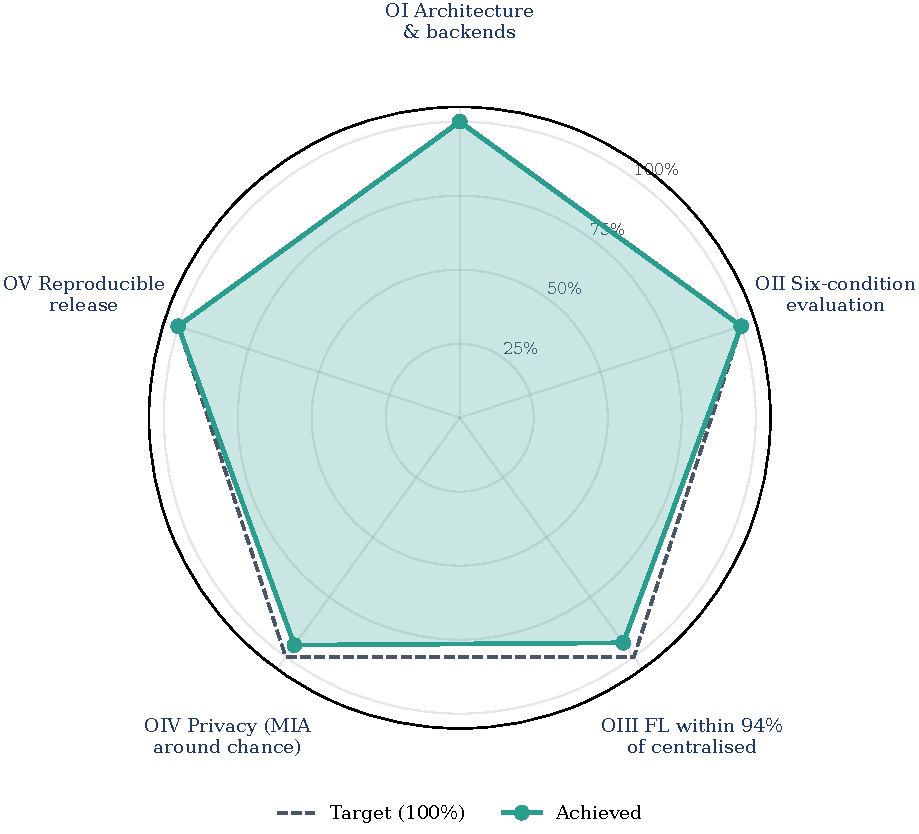
\includegraphics[width=0.78\linewidth]{res/fig-concept-objectives-radar.pdf}
    \caption[Objectives versus achievement]{Achievement against the five SMART objectives OI-OV (see Section~\ref{sec:meth:requirements} for the full statements). The shaded region is the self-assessed coverage of each objective by the delivered artefacts (codebase, benchmark, dissertation). OI-OIV are fully delivered; OV is delivered at the benchmark scale reported in Chapter~\ref{ch:results} and is identified as a candidate for larger-scale replication in future work. The figure supports the achievements analysis in Section~\ref{sec:concl:achievements}.}
    \label{fig:concept-objectives-radar}
\end{figure}

Taken together, the benchmark results are the central piece of first-party evidence that the three trilemma axes can be decoupled in this domain rather than traded against each other: the utility axis is held close to the centralised upper bound by the local RAG context, the efficiency axis collapses by nearly three orders of magnitude because only the low-rank adapter delta crosses the network boundary, and the privacy axis sits at the chance baseline because that delta is additionally Fernet-encrypted and reveals little to a threshold-based attacker. No single axis is optimised at the expense of the others; the composition is what matters, not any one component in isolation.

\section{Research Contribution}
\label{sec:concl:contribution}

Beyond the benchmark itself, the dissertation contributes three artefacts that are intended to be reusable outside the financial setting studied here. First, the composition of FLoRA-style adapter federation with a bank-scoped local RAG retriever, evaluated on the IBM AML task, is the novel design principle that makes the trilemma decoupling possible: the low-rank adapter carries the generalisable reasoning signal across institutions, while the local graph retriever carries the silo-specific structural signal that would otherwise have to be pooled centrally. The two reasoning substrates are complementary, and the benchmark isolates the individual contribution of each. Second, the Strategy-pattern graph-store layer, with concrete Kuzu, NetworkX, and Neo4j backends and a Neo4j path that is production-deployable, is a minimal and directly reusable abstraction for any federated RAG project that needs to swap between embedded, in-memory, and distributed graph stores without touching the federation or RAG code. Third, the archived dataset of per-round per-client metrics under \texttt{data/2026-04-02/}, together with the pinned \texttt{benchmark-2026-04-02} tag and the figure-regeneration scripts under \texttt{scripts/figures/}, gives downstream researchers a drop-in reference against which to measure re-implementations, parameter sweeps, or alternative aggregators on the same task.

\subsection*{Where to find the evidence for each objective}

For the convenience of a reader auditing the project against its five SMART objectives stated in Section~\ref{sec:meth:requirements}, this paragraph names the location of the supporting evidence for each.

\begin{itemize}
    \setlength\itemsep{0em}
    \item \textbf{OI (Architecture)} - the module layout (\texttt{src/data/}, \texttt{src/graph/}, \texttt{src/model/}, \texttt{src/pipeline/}, \texttt{src/federation/}, \texttt{src/security/}) and the Strategy-pattern graph layer are described in Section~\ref{sec:meth:arch} and Section~\ref{sec:meth:strategy}; the public repository is \url{https://github.com/SlaviXG/thinking-inside-the-box}.
    \item \textbf{OII (Simulation)} - the cross-silo simulation, the in-process federated loop, and the deviation from Flower's Virtual Client Engine are described in Section~\ref{sec:meth:impl} and Section~\ref{sec:meth:deviations}; the configuration table is Table~\ref{tab:config-summary}.
    \item \textbf{OIII (Benchmark)} - the six-condition matrix is reported in Chapter~\ref{ch:results}; the per-round JSON archive is under \texttt{data/2026-04-02/} at git tag \texttt{benchmark-2026-04-02} and is reproducible from the figure-regeneration scripts under \texttt{scripts/figures/}.
    \item \textbf{OIV (Trilemma measurement)} - utility (F1 score) is in Section~\ref{sec:results:utility}; efficiency (bytes and wall-clock) is in Section~\ref{sec:results:efficiency}; privacy (membership-inference AUC) is in Section~\ref{sec:results:privacy}. The trilemma summary is Table~\ref{tab:trilemma-summary}.
    \item \textbf{OV (Evidence)} - the headline numbers for FLoRA-with-RAG (peak F1 score $0.805$ within $0.05$ of the centralised upper bound, $882\times$ bandwidth reduction, MIA AUC in the $0.44$-$0.45$ band) are reported in Sections~\ref{sec:results:utility}, \ref{sec:results:efficiency}, and~\ref{sec:results:privacy}, and re-derived independently by the verification scripts under \texttt{scripts/verify/} (\texttt{verify\_comms\_volume.py}, \texttt{verify\_cost\_of\_misclassification.py}, \texttt{verify\_production\_deployment.py}). The radar chart in Figure~\ref{fig:concept-objectives-radar} summarises the achievement against the five objectives at a glance.
\end{itemize}

\section{Future Work}
\label{sec:concl:future}

Three extensions are identified as natural follow-ups. First, the LoRA adapter configuration was held at the FLoRA paper's defaults ($r=8$, \texttt{q\_proj}+\texttt{v\_proj}) for the benchmark reported here; the current code defaults ($r=16$ with the full attention block and two feed-forward projections, for approximately 32.5 million trainable parameters) are expected to raise the achievable F1 score at the cost of inflating the adapter payload to roughly 170~MB per client per round, approximately ten times the $r=8$ baseline but still nearly two orders of magnitude smaller than the classical FedAvg reference; a re-benchmark at those defaults would validate that expectation and sharpen the utility-versus-bandwidth trade-off curve reported in Chapter~\ref{ch:results}. Second, the membership inference attack is a threshold-based proxy rather than a shadow-model attack; a stronger attacker, implemented as a shadow-model ensemble following the Shokri et al. construction, would provide a more conservative privacy upper bound and place the near-chance AUC observed here in a more defensible context. Third, the evaluation is single-seed; reporting across several seeds would quantify cross-seed variance alongside the cross-round variance currently reported, turning the headline numbers from point estimates into confidence intervals without changing the architecture.

\section{Closing Reflection}

The thesis behind this project is that the three trilemma axes - utility, efficiency, and privacy - can be decoupled in a federated LLM pipeline rather than traded against each other, provided the reasoning substrate is separated from the knowledge substrate and the federation boundary carries only low-rank adapter deltas. The benchmark reported in Chapter~\ref{ch:results} is consistent with that thesis at the scale of three banks, a single Colab A100, and a ten-round budget. The same architecture is directly reusable in any setting where data must stay with its owner and the owner's reasoning must nevertheless benefit from a shared model - healthcare, legal discovery, inter-hospital research, cross-jurisdiction compliance - and the reproducibility artefacts shipped with this dissertation are intended to make that reuse a matter of configuration rather than of re-implementation.

% \section{Introduction}

% \subsection{Background and Motivation}
% Since its inception in 2017, Federated Learning (FL) has transformed how industries leverage sensitive data \cite{mcmahan2017communication}. By training models locally and sharing only weight updates, FL has enabled breakthrough applications in \textbf{Healthcare} (collaborative disease detection across hospitals), \textbf{Mobile Computing} (predictive text on smartphones), and \textbf{Finance} (inter-bank fraud detection). In the financial sector specifically, FL offers a unique opportunity to combat money laundering by aggregating patterns from multiple banks without violating strict data privacy regulations (e.g., GDPR).

% However, deploying Large Language Models (LLMs) in these federated environments introduces a fundamental \textbf{Trilemma} \cite{plosone2023e0338822}:
% \begin{enumerate}
%     \setlength\itemsep{0em} % Reduces space between items to save page space
%     \item \textbf{Privacy:} Keeping data local prevents centralized reasoning.
%     \item \textbf{Utility:} Local models often lack the ``global context'' required for complex fraud detection.
%     \item \textbf{Efficiency:} Transmitting massive LLM weights overwhelms network bandwidth.
% \end{enumerate}

% \begin{figure}[htbp]
%     \centering
%     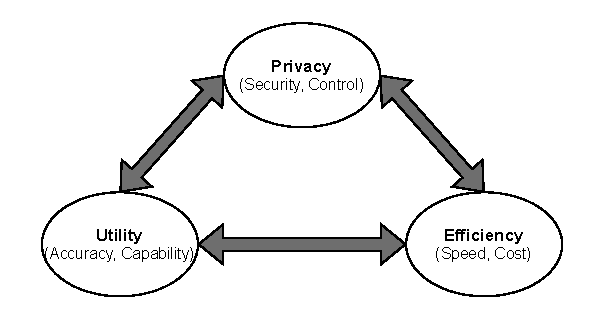
\includegraphics[width=0.6\linewidth]{res/federated_learning_trilemma.pdf}
%     \caption{The Federated Learning Trilemma: Traditional architectures force a trade-off. This project aims to \textbf{circumvent} this by decoupling reasoning from knowledge.}
%     \label{fig:fl_trilemma}
% \end{figure}

% \subsection{Proposed Solution}
% This project proposes a paradigm shift to \textbf{resolve} these conflicting objectives. By decoupling the ``Brain'' (Reasoning) from the ``Memory'' (Knowledge), we can train lightweight adapters to perform logic \cite{flora2024federated} while keeping all sensitive records in a secure, local Retrieval Augmented Generation (RAG) system \cite{lewis2021retrievalaugmentedgenerationknowledgeintensivenlp}.


% \subsection{Related Work}
% The key background sources that enable and justify this novel approach are presented and categorised below.

% \begin{table*}[htbp]
% \centering
% \caption{Key References Supporting the Proposed Architecture (Categorized)}
% \label{tab:related_work}
% \renewcommand{\arraystretch}{1.3}
% \begin{tabularx}{\textwidth}{p{2.2cm} p{3.2cm} p{3.8cm} X}
% \toprule
% \textbf{Category} & \textbf{Source} & \textbf{Key Concept} & \textbf{Relevance to Project} \\
% \midrule

% \textbf{Theoretical Foundation} & 
% Zhou et al. (2023), \textit{DualMask: Federated Optimization of Trilemma \cite{plosone2023e0338822}} & 
% Formally defines the ``Trilemma'' in Federated Learning, where privacy, model accuracy, and system efficiency conflict. & 
% Provides the theoretical problem statement that the ``Thinking Inside the Box'' architecture aims to resolve. \\
% \midrule

% \textbf{Theoretical Foundation} & 
% Allouah et al. (2023), \textit{On the Privacy--Robustness--Utility Trilemma \cite{allouah2023trilemma}} & 
% Analyzes trade-offs in distributed systems, particularly robustness against adversarial attacks. & 
% Justifies why the architecture (which keeps raw data offline) is resilient to data poisoning and leakage. \\
% \midrule

% \textbf{Architectural Components} & 
% DeepSeek-AI et al. (2025), \textit{DeepSeek-R1: Incentivizing Reasoning Capability \cite{deepseek2025r1}} & 
% Introduces ``Reasoning Models'' that use Chain-of-Thought (CoT) to solve complex logic puzzles rather than just predicting words. & 
% This model class is utilised to enable ``local investigation'' capabilities that standard LLMs lack. \\
% \midrule

% \textbf{Architectural Components} & 
% Lewis et al. (2020), \textit{Retrieval-Augmented Generation (RAG) \cite{lewis2021retrievalaugmentedgenerationknowledgeintensivenlp}} & 
% Establishes the RAG framework for connecting LLMs to external databases. & 
% Basis for the ``External Memory'' component, allowing secure access to private bank data without training on it. \\
% \midrule

% \textbf{Efficiency Mechanisms} & 
% Hu et al. (2022), \textit{LoRA: Low-Rank Adaptation of LLMs \cite{hu2021lora}} & 
% Introduces efficient fine-tuning by updating only a small subset of parameters via low-rank decomposition. & 
% Core enabler of the architecture, allowing transmission of tiny ``adapters'' instead of massive model weights. \\
% \midrule

% \textbf{Efficiency Mechanisms} & 
% Wang et al. (2024), \textit{FLORA: Federated Low-Rank Adaptation \cite{flora2024federated}} & 
% Extends low-rank adaptation to federated settings, optimizing communication efficiency while maintaining model performance. & 
% Strengthens the deployment strategy by reducing communication overhead and preserving personalisation. \\

% \bottomrule
% \end{tabularx}
% \end{table*}


% \section{Aim and Objectives}

% \subsection{Aim}
% This project aims to design and evaluate a privacy-preserving architecture integrating \textbf{Low-Rank Adaptation (FLoRA)} \cite{flora2024federated} and \textbf{Retrieval Augmented Generation (RAG)} \cite{lewis2021retrievalaugmentedgenerationknowledgeintensivenlp}. By decoupling reasoning from knowledge, the system seeks to resolve the ``Privacy-Utility-Efficiency Trilemma'' in financial forensics, enabling distributed fraud detection on the \textbf{IBM AML dataset} \cite{weber2018scalablegraphlearningantimoney} without exposing raw transaction data.

% \subsection{Objectives}
% To achieve this, the project needs to meet the following objectives:
% \begin{enumerate}
%     \setlength\itemsep{0em} % Tightens the list
%     \item \textbf{Develop a Federated Simulation:} Utilise \textbf{Flower} \cite{beutel2022flowerfriendlyfederatedlearning} to simulate a cross-silo network of banking institutions using the \textbf{IBM AML dataset} \cite{weber2018scalablegraphlearningantimoney}, explicitly modeling realistic heterogeneous (non-IID) data distributions.
    
%     \item \textbf{Implement Local RAG:} Integrate on-device \textbf{Retrieval Augmented Generation} \cite{lewis2021retrievalaugmentedgenerationknowledgeintensivenlp} to enable local models to query private transaction logs for reasoning. This ensures enhanced fraud detection capabilities while raw data remains strictly local.
    
%     \item \textbf{Evaluate via the ``Trilemma'' Framework:} Benchmark the architecture against baselines across \textbf{Utility} (F1-Score \cite{10.3115/1072064.1072067}), \textbf{Efficiency} (Communication Volume, Latency), and \textbf{Privacy} (Resilience to data leakage), validating the effective resolution of the trade-off.
% \end{enumerate}


% \section{Planning}

% \subsection{Work Plan}
% The project follows a linear \textbf{technical} execution path, supported by \textbf{parallel documentation streams}. This ``Simulation-First'' strategy ensures that hardware risks are mitigated while writing tasks (Poster and Thesis drafting) occur concurrently with experimental phases. The schedule is aggressively front-loaded to ensure the core technical implementation is completed by March 20th.

% \begin{figure}[H]
%     \centering
%     % Make sure the filename matches exactly what you uploaded
%     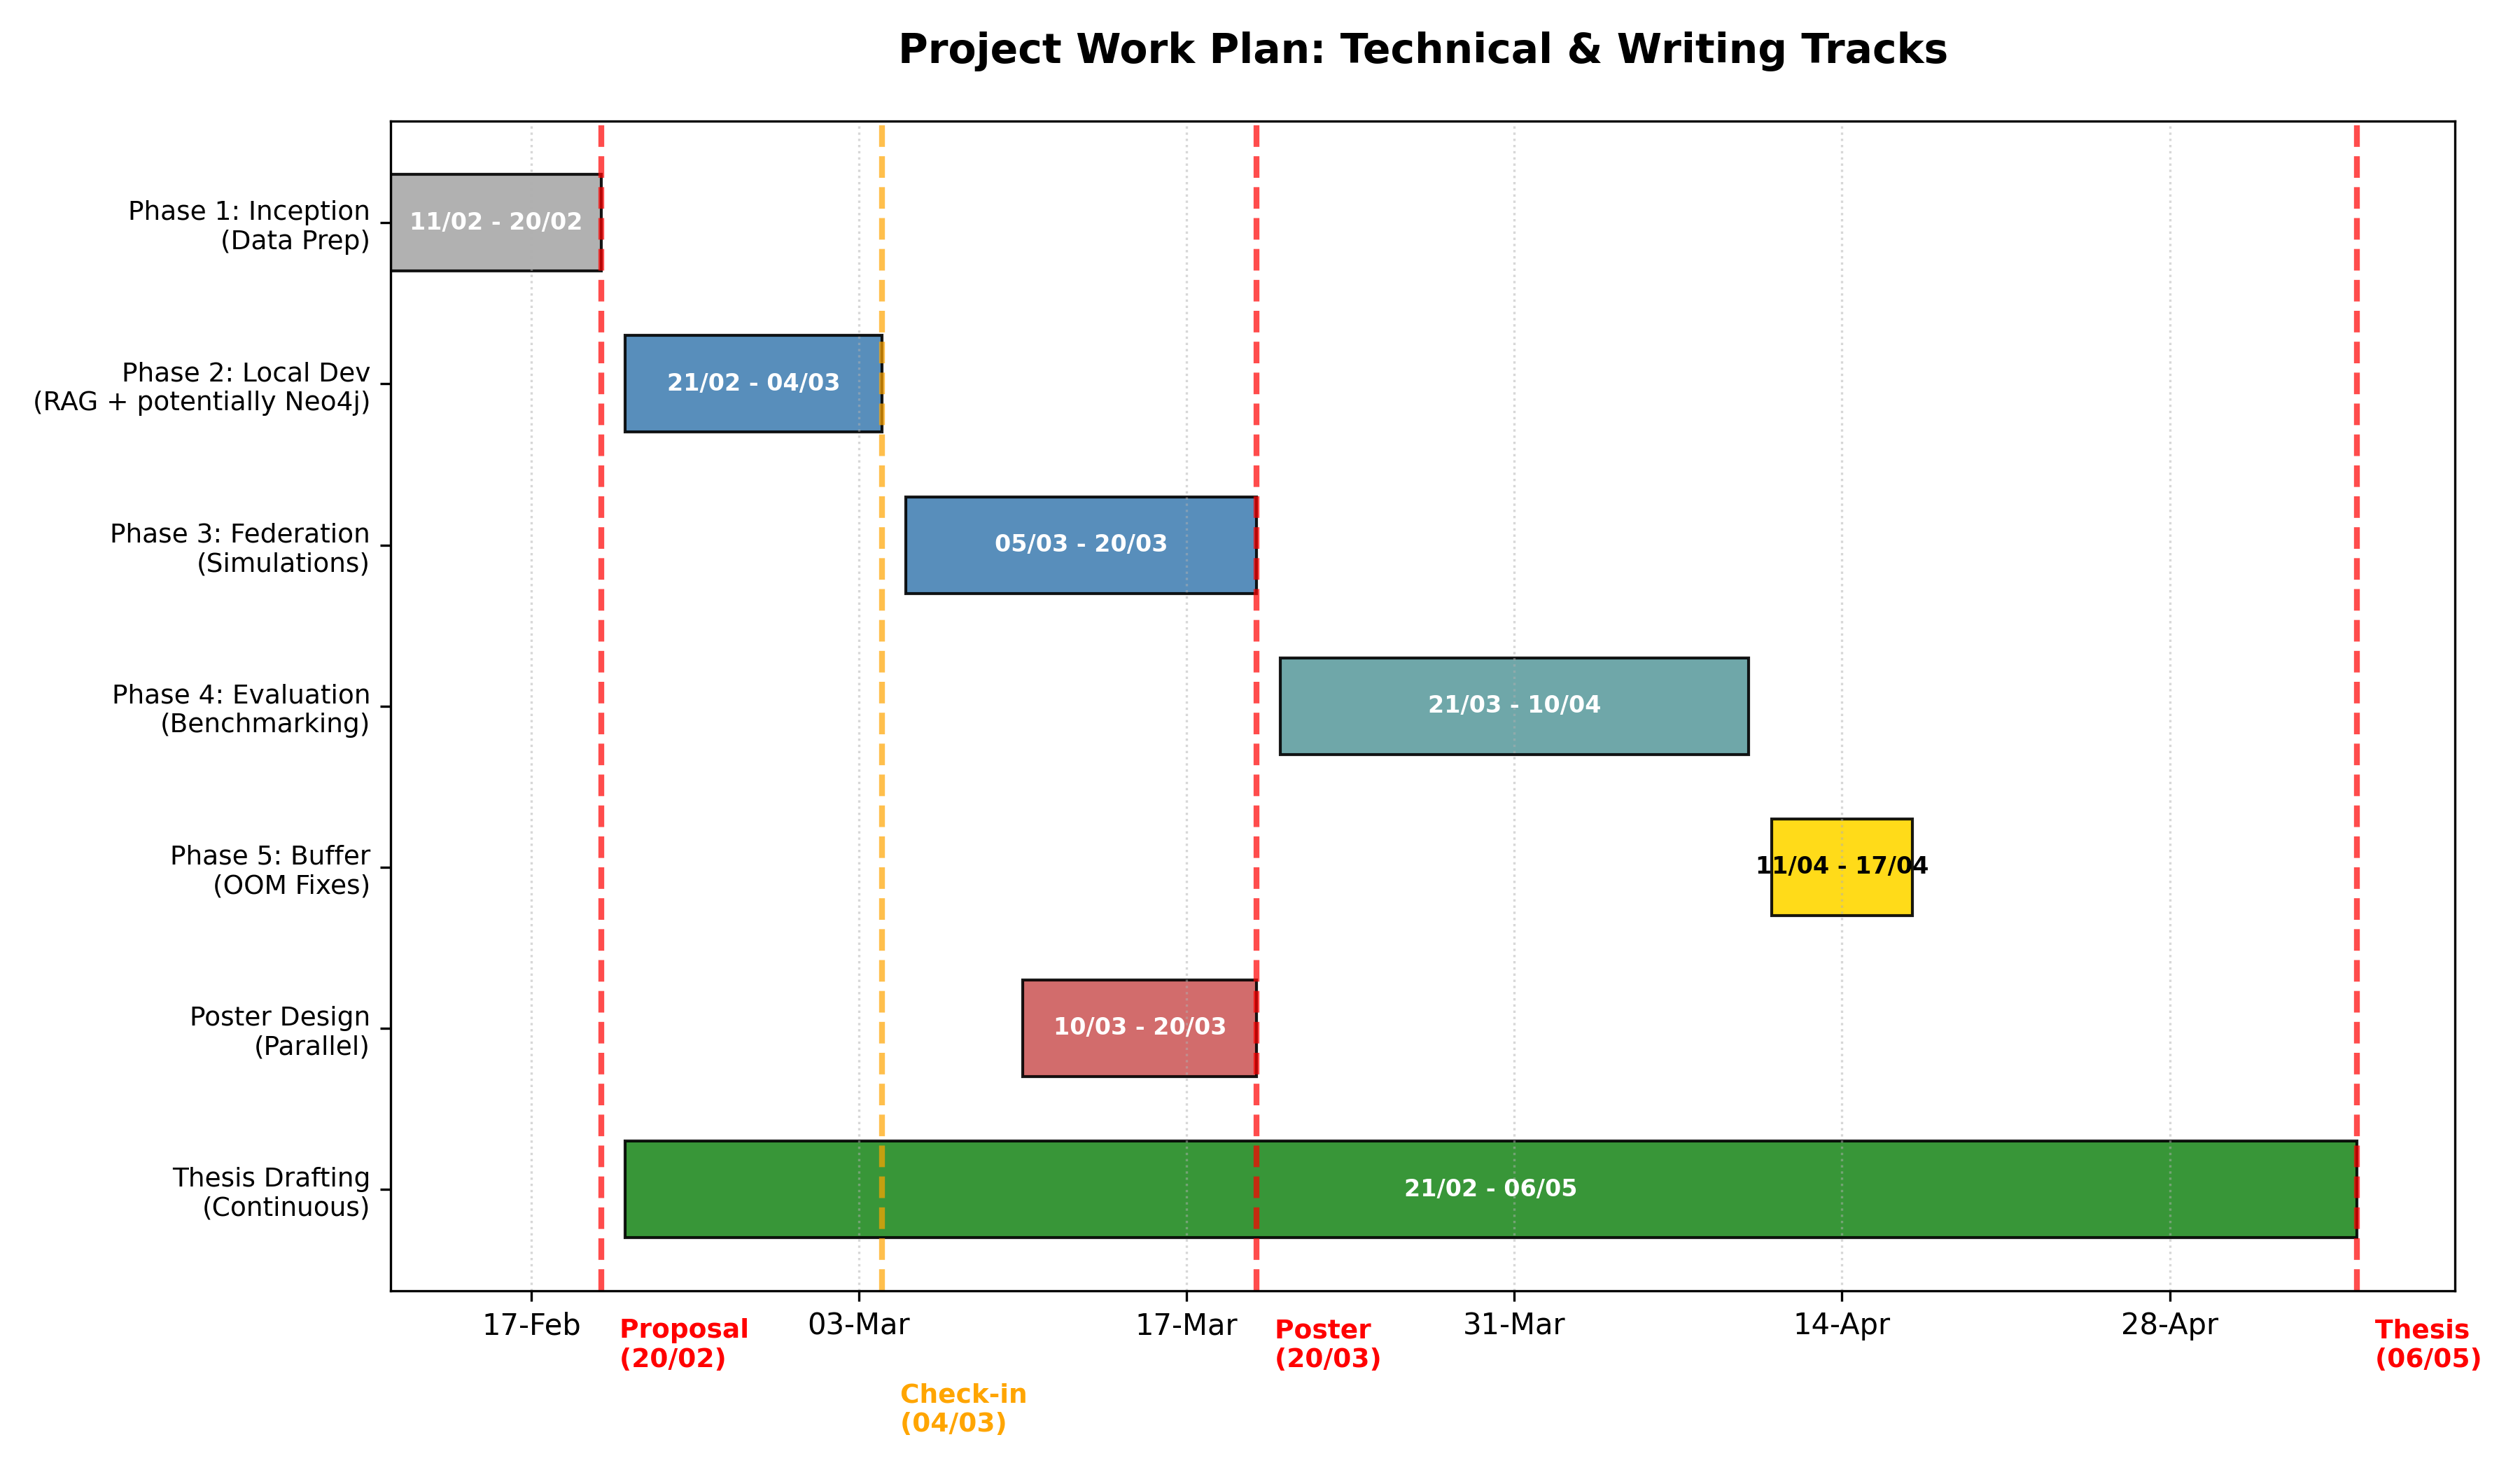
\includegraphics[width=1\textwidth]{res/gantt_chart_parallel.png}
%     \caption{Project Gantt Chart showing parallel Technical and Writing tracks with buffer contingency.}
%     \label{fig:gantt_chart}
% \end{figure}

% \subsection{Methodology}

% \subsubsection{Simulation-First Architecture}
% The plan is structured around a ``Simulation-First'' methodology. Rather than attempting to deploy immediately to distributed hardware, Phase 2 focuses entirely on establishing a working \textbf{Local RAG} system. This isolates the complexity of ``Reasoning'' from the complexity of ``Networking.'' Only once the model can successfully generate valid queries on a single node (Milestone M2) will the \textbf{Flower} federation layer be introduced in Phase 3. This dependency structure ensures that the Poster deadline (Mar 20) can be met with a working prototype, even if the federation experiments require further tuning during the evaluation phase.

% \subsubsection{Resource Plan}
% To ensure viability within the timeline, the project primarily relies on accessible, free-tier resources:
% \begin{itemize}
%   \item \textbf{Compute:} Google Colab (Tesla T4 GPU, 16GB VRAM \cite{nvidia2018t4}) is sufficient for the target model (DeepSeek-R1-Distill-8B \cite{deepseek2025r1}) using 4-bit quantization ($\sim$6GB VRAM load).
%   \item \textbf{Software Stack:} The Flower framework's ``Virtual Client Engine'' allows for the serial simulation of multiple banks on a single GPU, removing the need for physical multi-node hardware \cite{beutel2022flowerfriendlyfederatedlearning}.
%   \item \textbf{Data Strategy:} The IBM AML Dataset is synthetic and open-source, eliminating ethical clearance delays associated with real banking data \cite{weber2018scalablegraphlearningantimoney}.
% \end{itemize}

% \subsubsection{Contingency Planning}
% A dedicated Buffer Week (Apr 11 – 17) is allocated between the Evaluation and final Write-up phases. This contingency is specifically reserved for resolving ``Out-Of-Memory'' (OOM) errors that frequently occur when scaling from local execution to federated simulation. If Phase 3 runs over schedule, the scope of the Evaluation can be reduced by removing the ``Centralized Control'' comparison, ensuring the core objectives are still met by the deadline.

% \subsubsection{Risks and Mitigation}
% The following risks have been identified based on the constraints of the Google Colab environment and the experimental nature of ``Reasoning'' models.

% \begin{itemize}
%     \setlength\itemsep{0.5em} % Adds space between the main bullet points for clarity

%     \item \textbf{Risk 1: Technical (Resource Limits) -- Significance: High} \\
%     The System RAM on Google Colab \cite{bisong2019google} is a hard bottleneck. Loading the full IBM transaction graph while simultaneously running the LLM may cause the session to crash (Out-Of-Memory).
%     \\[0.5em] % Adds a small gap before the mitigation
%     \textbf{Mitigation:} Utilise a low-resolution dataset. Use \textbf{4-bit Quantization (QLoRA)} to reduce the model's VRAM footprint to $\sim$6GB \cite{dettmers2024qlora}.

%     \item \textbf{Risk 2: Methodological (Simulation Fidelity) -- Significance: Medium} \\
%     A single-machine simulation does not inherently capture the network latency, packet loss, or straggler behavior of a real-world distributed system.
%     \\[0.5em]
%     \textbf{Mitigation:} Introduce artificial time delays and Gaussian noise within the Flower aggregation loop. This mathematically models heterogeneous network conditions, ensuring the evaluation metrics reflect a realistic deployment scenario.

%     \item \textbf{Risk 3: Model Reliability (AI Safety) -- Significance: Medium} \\
%     ``Reasoning'' models can hallucinate, producing invalid database interaction syntax (e.g., non-existent relationship types), which would crash the execution pipeline during automated testing.
%     \\[0.5em]
%     \textbf{Mitigation:} Evaluate the system against safety metrics. Implement a deterministic Syntax Validator (Linter) middleware. Invalid queries will be caught pre-execution and flagged as ``Reasoning Failures'' for the Utility metric, allowing the simulation to continue without crashing.

% \end{itemize}

\bibliographystyle{alpha}
\bibliography{sample}

\end{document}